%%%%%%%%%%%%%%%%%%%%%%%%%%%%%%%%%%%%%%%%%%  不使用 authblk 包制作标题  %%%%%%%%%%%%%%%%%%%%%%%%%%%%%%%%%%%%%%%%%%%%%%
%-------------------------------PPT Title-------------------------------------
\title{\rm{Material~Studio}软件使用简介}
%-----------------------------------------------------------------------------

%----------------------------Author & Date------------------------------------
%\author[\textrm{Jun\_Jiang}]{姜\;\;骏\inst{}} %[]{} (optional, use only with lots of authors)
%% - Give the names in the same order as the appear in the paper.
%% - Use the \inst{?} command only if the authors have different
%%   affiliation.
%\institute[BCC]{\inst{}%
%\institute[Gain~Strong]{\inst{}%
%\vskip -20pt 北京市计算中心~云平台事业部~姜骏}
%\vskip -20pt {\large 格致斯创~科技}
\date[\today] % (optional, should be abbreviation of conference name)
{	%{\fontsize{6.2pt}{4.2pt}\selectfont{\textcolor{blue}{E-mail:~}\url{jiangjun@bcc.ac.cn}}}
\vskip 45 pt {\fontsize{8.2pt}{6.2pt}\selectfont{%北京科技大学% 报告地点
	\vskip 5 pt \textrm{2024.04.09}}}
}

%% - Either use conference name or its abbreviation
%% - Not really information to the audience, more for people (including
%%   yourself) who are reading the slides onlin%%   yourself) who are reading the slides onlin%%   yourself) who are reading the slides onlineee
%%%%%%%%%%%%%%%%%%%%%%%%%%%%%%%%%%%%%%%%%%%%%%%%%%%%%%%%%%%%%%%%%%%%%%%%%%%%%%%%%%%%%%%%%%%%%%%%%%%%%%%%%%%%%%%%%%%%%

\subject{}
% This is only inserted into the PDF information catalog. Can be left
% out.
%\maketitle
\frame
{
%	\frametitle{\fontsize{9.5pt}{5.2pt}\selectfont{\textcolor{orange}{“高通量并发式材料计算算法与软件”年度检查}}}
\titlepage
}
%-----------------------------------------------------------------------------

%------------------------------------------------------------------------------列出全文 outline ---------------------------------------------------------------------------------
\section*{}
\frame[allowframebreaks]
{
  \frametitle{Outline}
%  \frametitle{\textcolor{mycolor}{\secname}}
  \tableofcontents%[current,currentsection,currentsubsection]
}
%%在每个section之前列出全部Outline
%%类似的在每个subsection之前列出全部Outline是\AtBeginSubsection[]
%\AtBeginSection[]
%{
%  \frame<handout:0>%[allowframebreaks]
%  {
%    \frametitle{Outline}
%%全部Outline中,本部分加亮
%    \tableofcontents[current,currentsection]
%  }
%}

%-----------------------------------------------PPT main Body------------------------------------------------------------------------------------
\small
%-----------------------------------------------------------------------------------------------------------------------------------------------------------------------%
%\section{计算示例:~\rm{Materials~Studio}}
\section{\rm{Materials~Studio}的安装}
\frame
{
	\frametitle{\textrm{Materials~Studio}的安装}
\begin{figure}[h!]
	\vspace{-10pt}
\centering
%\caption{\tiny \textrm{The Nolbel Prize in Chemistry 1998 Summary.}}%(与文献\cite{EPJB33-47_2003}图1对比)
\includemovie[poster, controls, mouse, url]{0.9\textwidth}{0.56\textwidth}{Figures/BIOVIA-Materials_Studio-Installation-Video-on-Windows.mp4}     %
\label{Materials-Studio_Install}
\end{figure}
}

\frame
{
	\frametitle{\textrm{MS}的架构}
\begin{figure}[h!]
\centering
\vspace*{-0.10in}
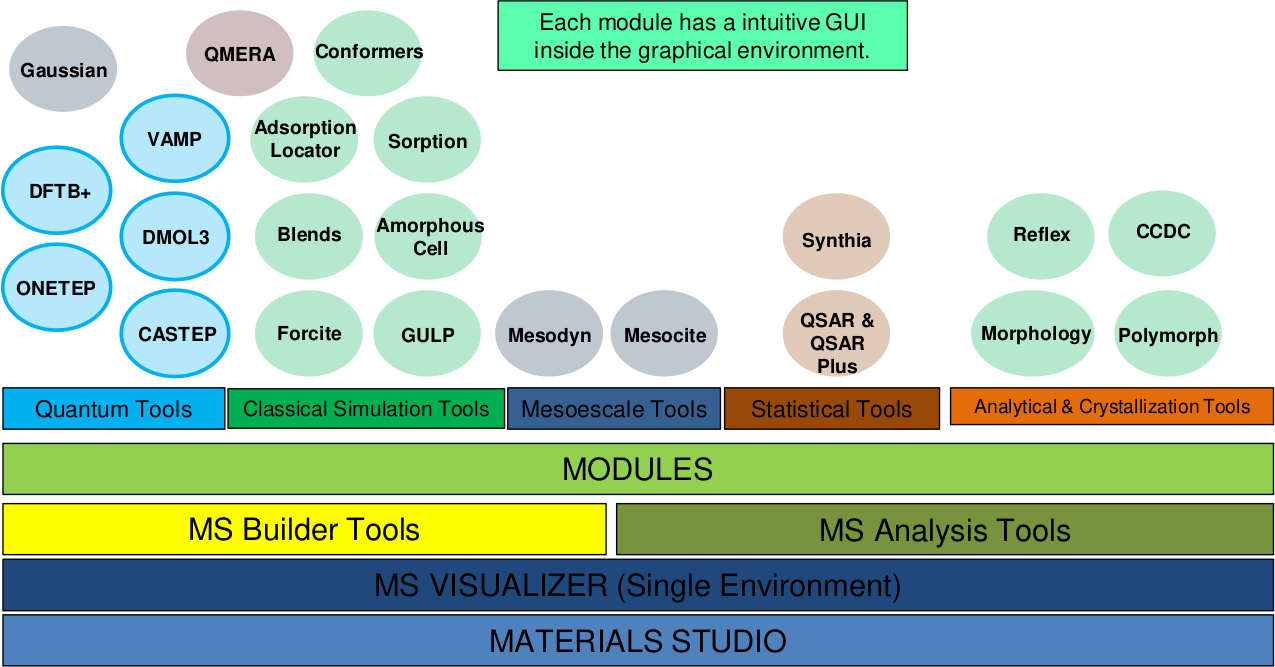
\includegraphics[height=2.20in,width=4.15in,viewport=0 0 1275 667,clip]{Figures/MS-main_Struct.png}
\caption{\tiny \textrm{The main structure of Materials studio.}}%(与文献\cite{EPJB33-47_2003}图1对比)
\label{MS-main-structure}
\end{figure}
}

\section{\rm{Materials~Studio:~Quick Start}}
\frame
{
	\frametitle{\textrm{MS:~Quick Start-01}}
\begin{figure}[h!]
\centering
\vspace*{-0.21in}
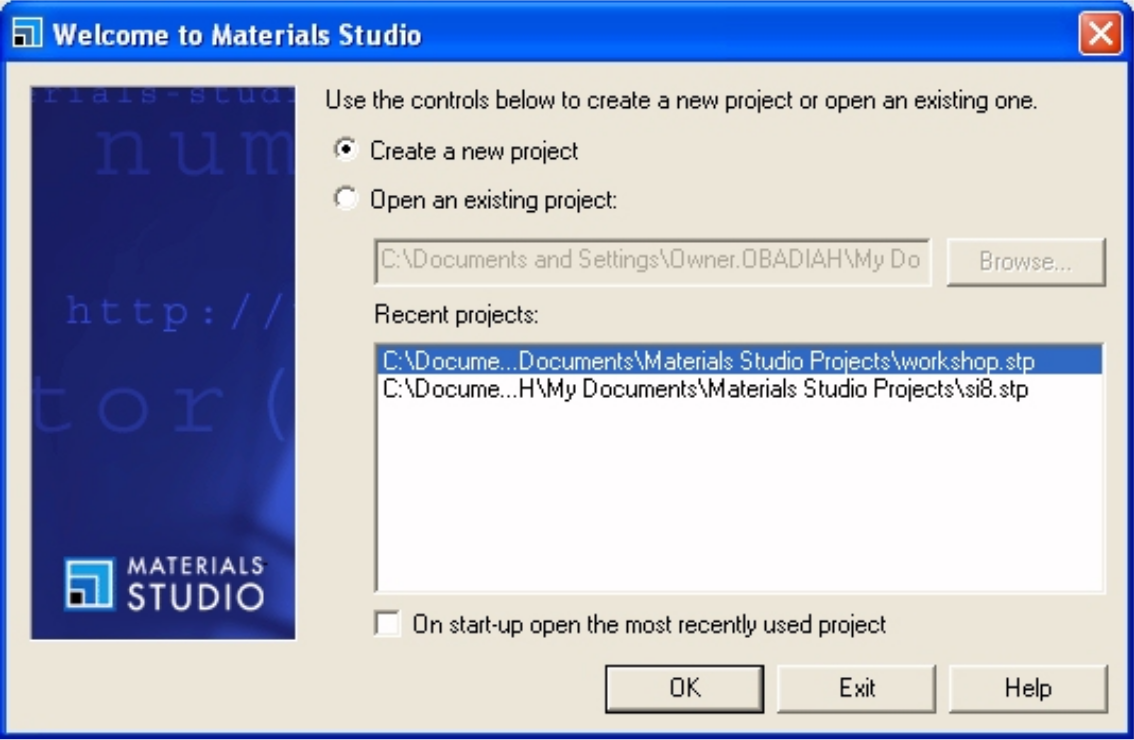
\includegraphics[height=2.70in,width=4.10in,viewport=0 0 1134 740,clip]{Figures/MS-New_Project-01.png}
\caption{\tiny \textrm{Quick Start for Materials studio:~Step-01.}}%(与文献\cite{EPJB33-47_2003}图1对比)
\label{MS-Quick_Start-01}
\end{figure}
}

\frame
{
	\frametitle{\textrm{MS:~Quick Start-02}}
\begin{figure}[h!]
\centering
\vspace*{-0.10in}
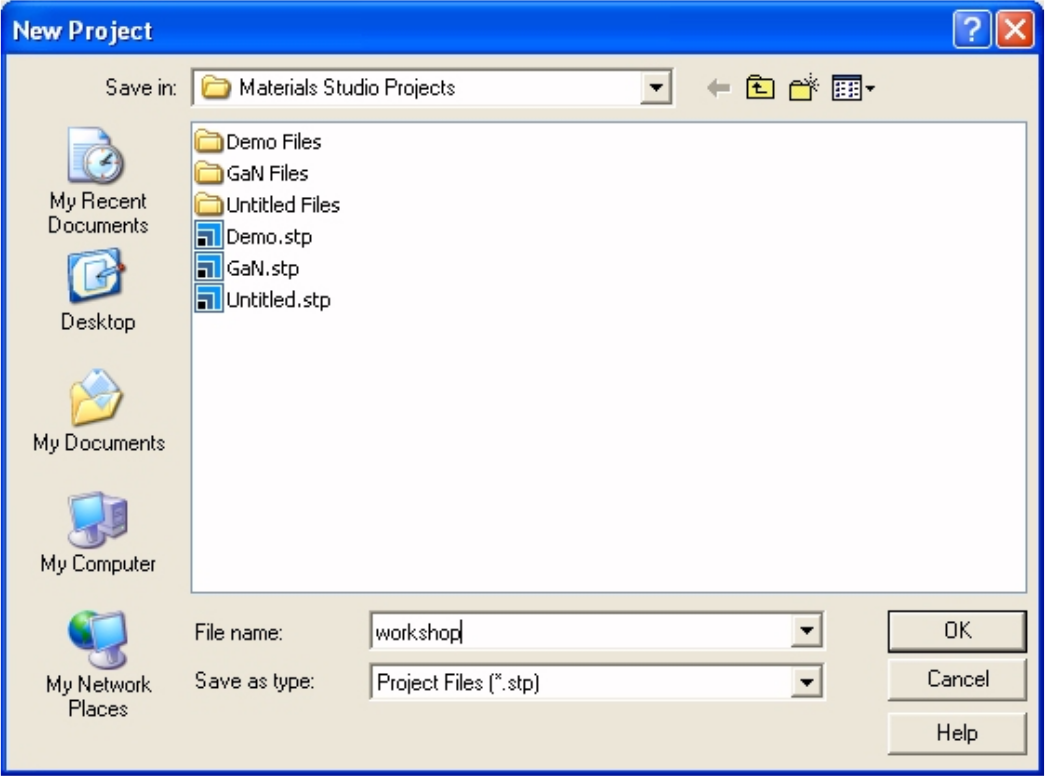
\includegraphics[height=2.70in,width=4.00in,viewport=0 0 1045 776,clip]{Figures/MS-New_Project-02.png}
\caption{\tiny \textrm{Quick Start for Materials studio:~Step-02.}}%(与文献\cite{EPJB33-47_2003}图1对比)
\label{MS-Quick_Start-02}
\end{figure}
}

\frame
{
	\frametitle{\textrm{MS:~Quick Start-03}}
\begin{figure}[h!]
\centering
\vspace*{-0.10in}
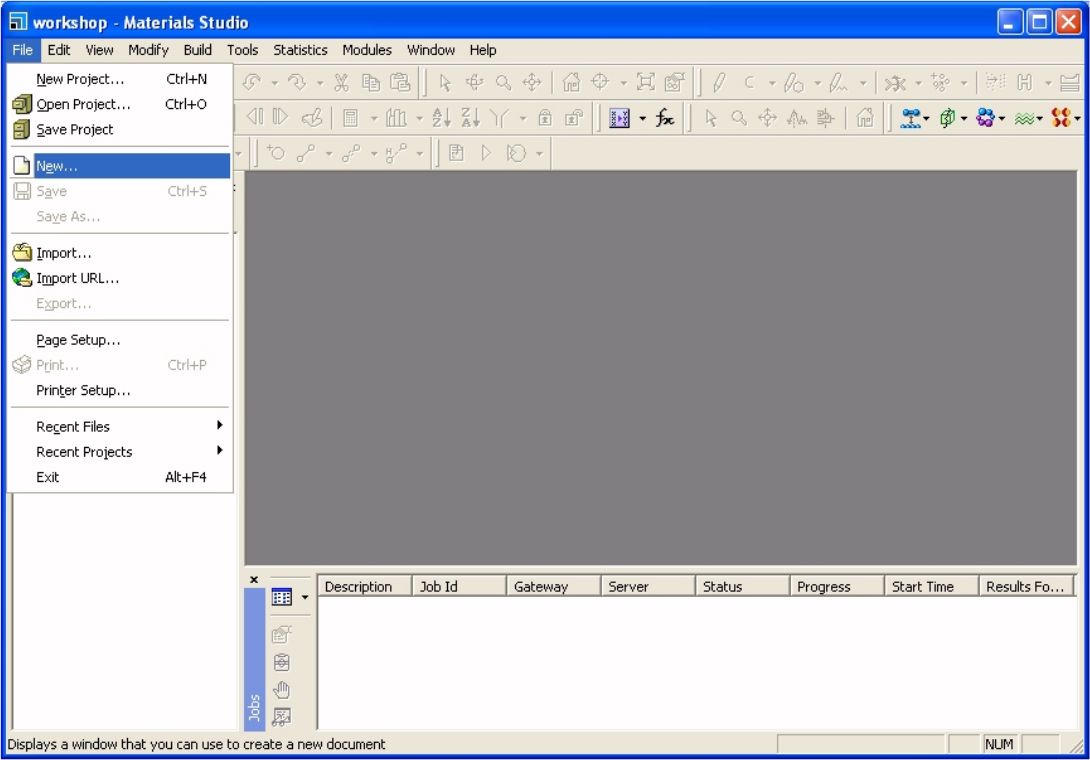
\includegraphics[height=2.68in,width=4.00in,viewport=0 0 1090 760,clip]{Figures/MS-New_Project-03.png}
\caption{\tiny \textrm{Quick Start for Materials studio:~Step-03.}}%(与文献\cite{EPJB33-47_2003}图1对比)
\label{MS-Quick_Start-03}
\end{figure}
}

%\subsection{\rm{Materials Studio:~Modelling}}
\frame
{
	\frametitle{\textrm{MS:~Quick Start-Modelling-01}}
\begin{figure}[h!]
\centering
\vspace*{-0.10in}
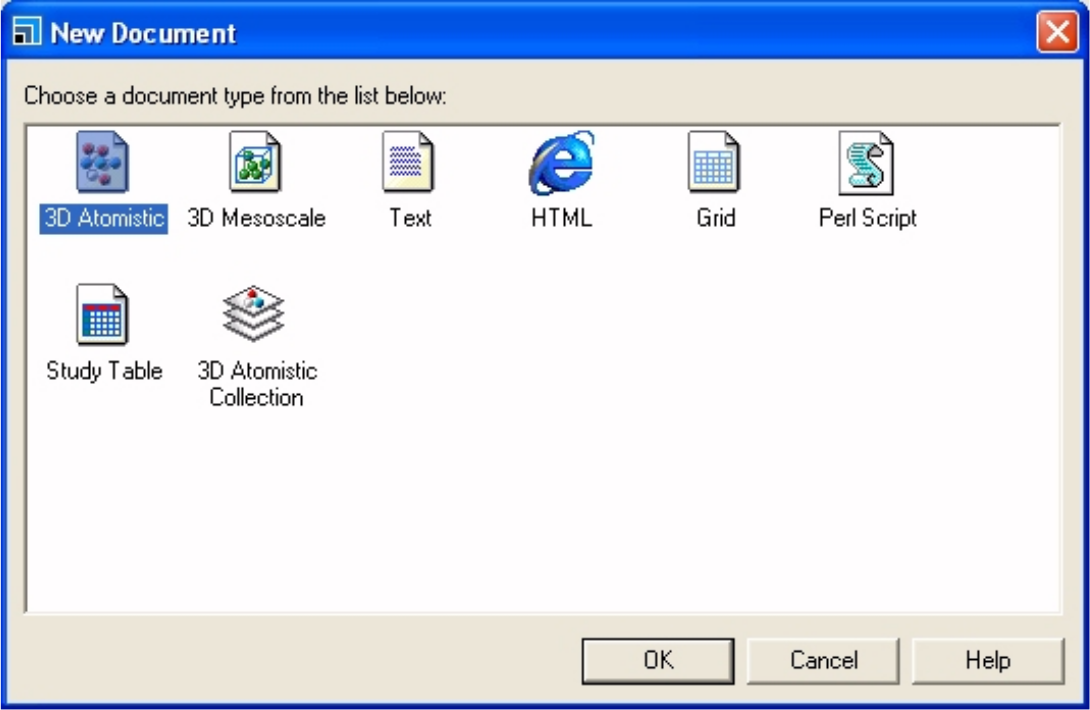
\includegraphics[height=2.60in,width=4.00in,viewport=0 0 1090 710,clip]{Figures/MS-New_Project-04.png}
\caption{\tiny \textrm{Quick Start for Materials studio:~Modelling-01.}}%(与文献\cite{EPJB33-47_2003}图1对比)
\label{MS-Quick_Start-Modelling-01}
\end{figure}
}

\frame
{
	\frametitle{\textrm{MS:~Quick Start-Modelling-02}}
\begin{figure}[h!]
\centering
\vspace*{-0.10in}
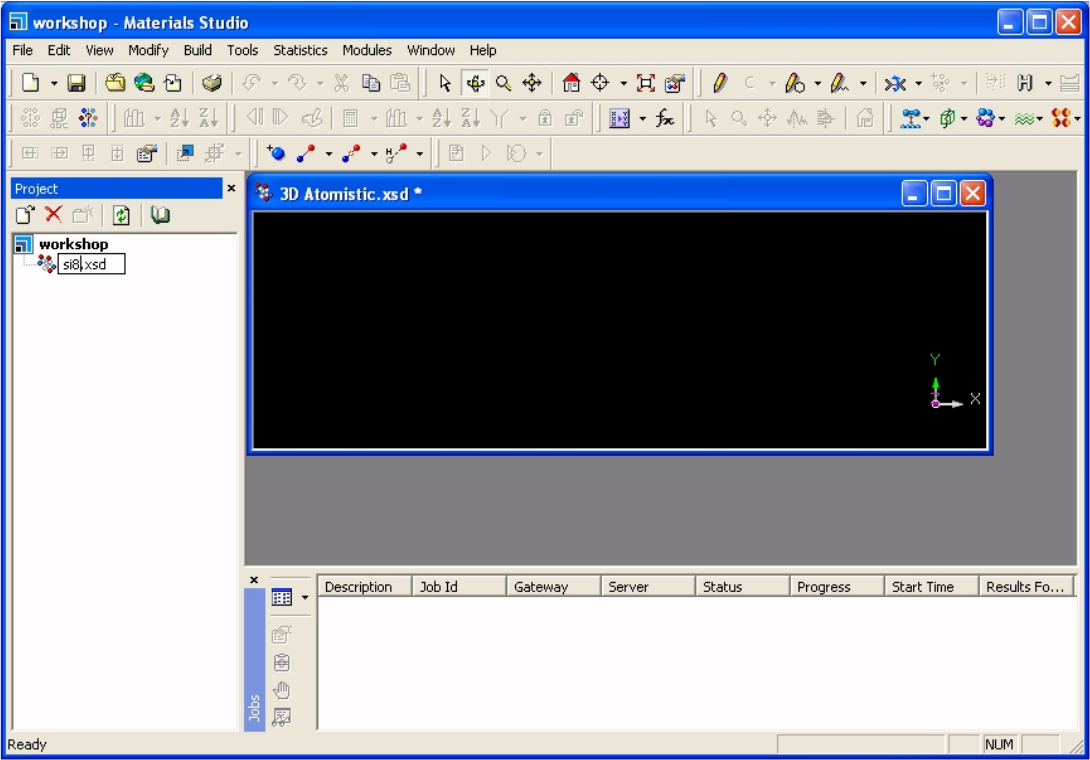
\includegraphics[height=2.68in,width=4.00in,viewport=0 0 1090 760,clip]{Figures/MS-New_Project-05.png}
\caption{\tiny \textrm{Quick Start for Materials studio:~Modelling-02.}}%(与文献\cite{EPJB33-47_2003}图1对比)
\label{MS-Quick_Start-Modelling-02}
\end{figure}
}

\frame
{
	\frametitle{\textrm{MS:~Modelling Crystal-01}}
\begin{figure}[h!]
\centering
\vspace*{-0.10in}
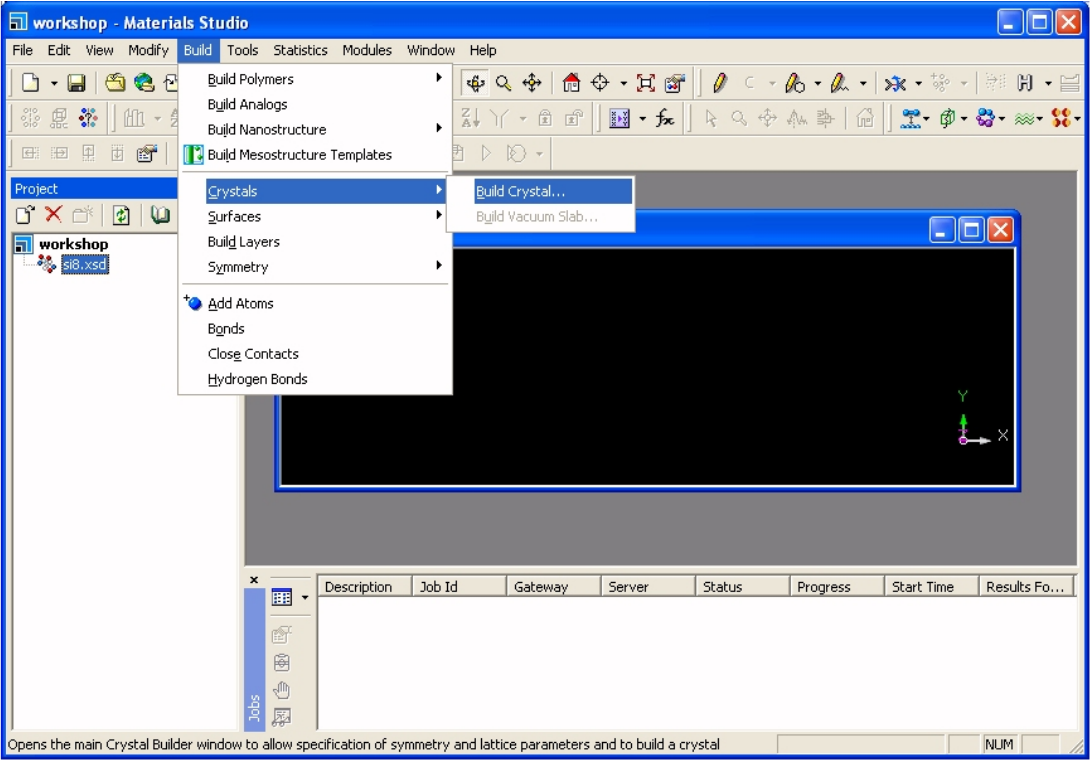
\includegraphics[height=2.68in,width=4.00in,viewport=0 0 1090 760,clip]{Figures/MS-New_Project-06.png}
\caption{\tiny \textrm{Modelling crystal by Materials studio.}}%(与文献\cite{EPJB33-47_2003}图1对比)
\label{MS-Modelling-Crystal-01}
\end{figure}
}

\frame
{
	\frametitle{\textrm{MS:~Modelling Crystal-02}}
\begin{figure}[h!]
\centering
\vspace*{-0.15in}
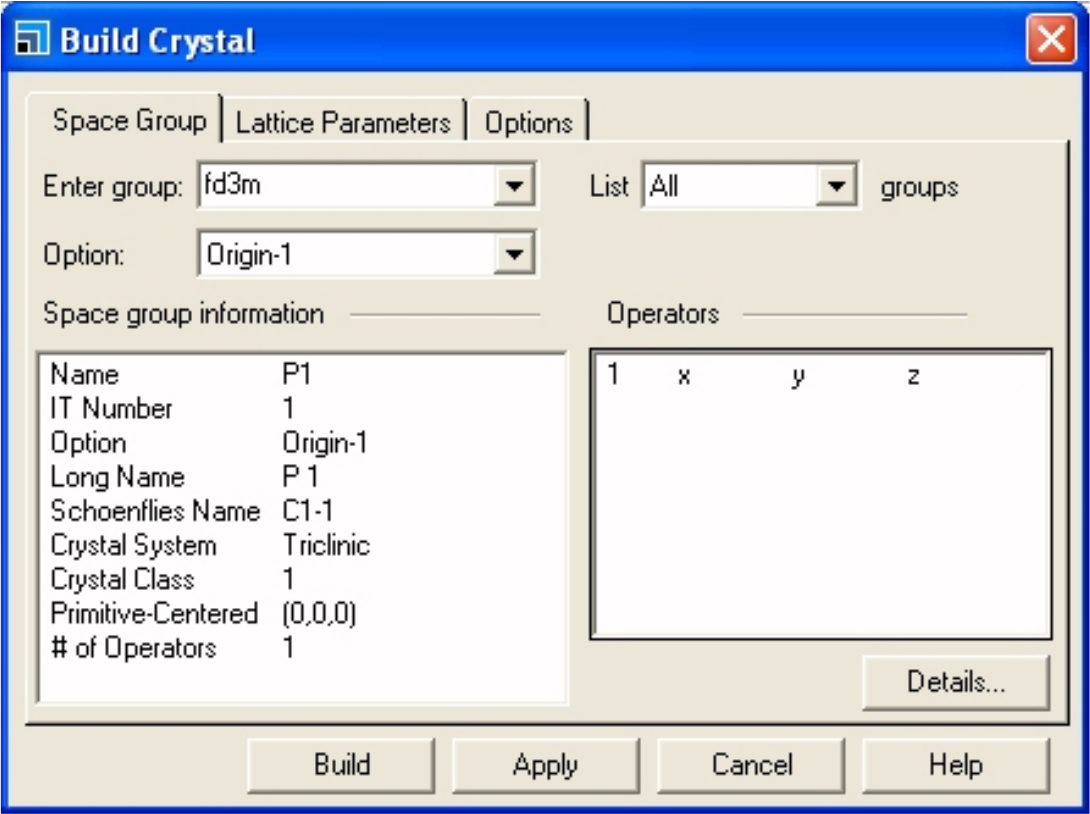
\includegraphics[height=2.75in,width=4.00in,viewport=0 0 1090 814,clip]{Figures/MS-New_Project-07.png}
\caption{\tiny \textrm{Modelling crystal by Materials studio:~Parameters.}}%(与文献\cite{EPJB33-47_2003}图1对比)
\label{MS-Modelling-Crystal-02}
\end{figure}
}

\frame
{
	\frametitle{\textrm{MS:~Modelling Crystal-03}}
\begin{figure}[h!]
\centering
\vspace*{-0.15in}
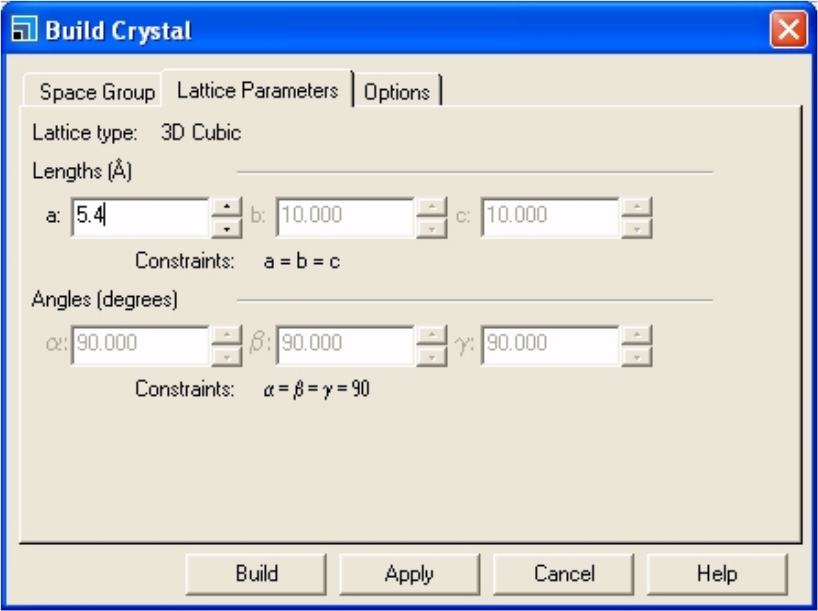
\includegraphics[height=2.75in,width=3.70in,viewport=0 0 818 616,clip]{Figures/MS-New_Project-08.png}
\caption{\tiny \textrm{Modelling crystal by Materials studio:~Lattice-parameters.}}%(与文献\cite{EPJB33-47_2003}图1对比)
\label{MS-Modelling-Crystal-03}
\end{figure}
}

\frame
{
	\frametitle{\textrm{MS:~Modelling Crystal-04}}
\begin{figure}[h!]
\centering
\vspace*{-0.10in}
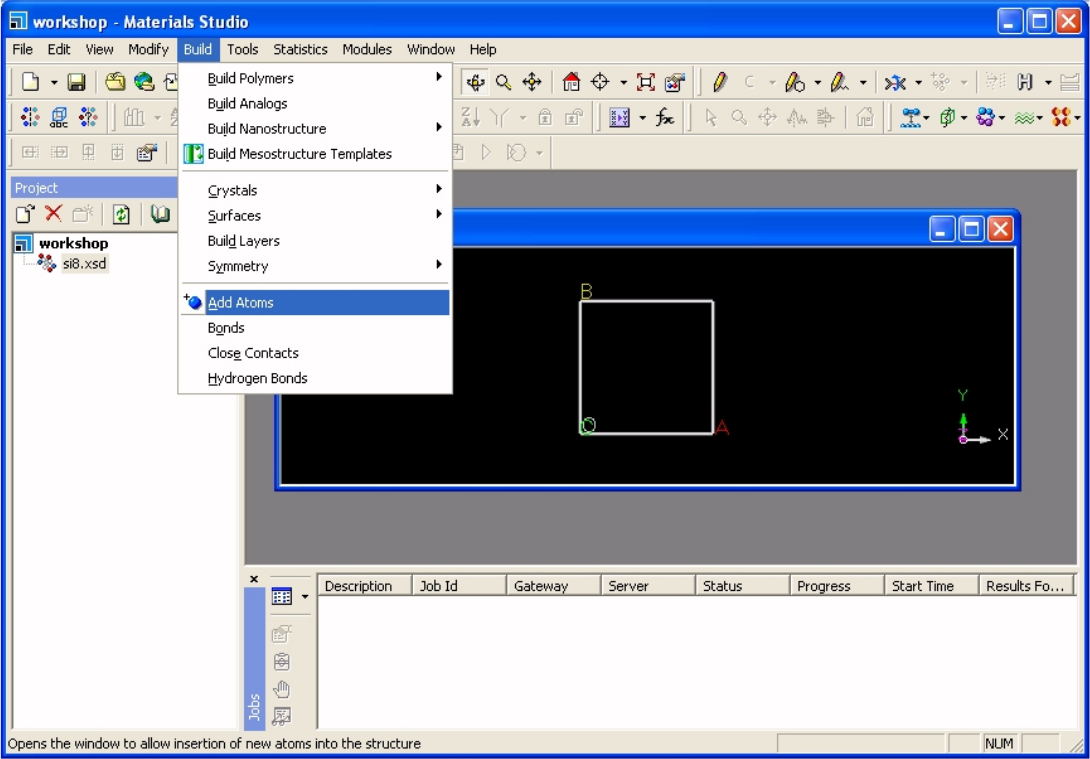
\includegraphics[height=2.70in,width=4.00in,viewport=0 0 1090 759,clip]{Figures/MS-New_Project-09.png}
\caption{\tiny \textrm{Modelling crystal by Materials studio:~Elements.}}%(与文献\cite{EPJB33-47_2003}图1对比)
\label{MS-Modelling-Crystal-04}
\end{figure}
}

\frame
{
	\frametitle{\textrm{MS:~Modelling Crystal example:~Si}}
\begin{figure}[h!]
\centering
\vspace*{-0.10in}
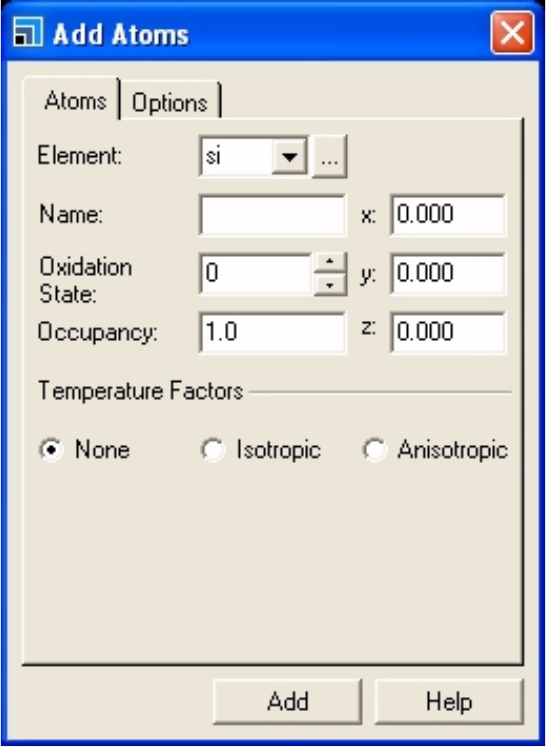
\includegraphics[height=2.70in,width=2.30in,viewport=0 0 546 747,clip]{Figures/MS-New_Project-10-Si_example.png}
\caption{\tiny \textrm{Modelling crystal by Materials studio:~Si.}}%(与文献\cite{EPJB33-47_2003}图1对比)
\label{MS-Modelling-Crystal-05}
\end{figure}
}

\frame
{
	\frametitle{\textrm{MS:~Modelling Crystal example:~Si}}
\begin{figure}[h!]
\centering
\vspace*{-0.10in}
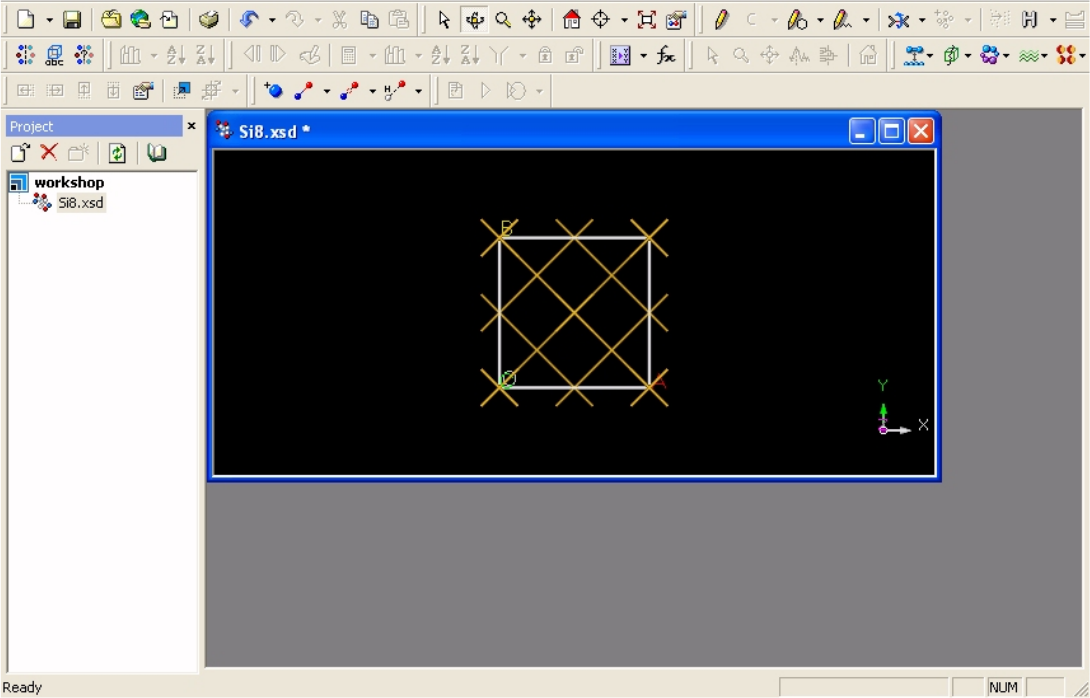
\includegraphics[height=2.65in,width=4.00in,viewport=0 0 1090 698,clip]{Figures/MS-New_Project-11-Si_crystal.png}
\caption{\tiny \textrm{Modelling crystal by Materials studio:~Si.}}%(与文献\cite{EPJB33-47_2003}图1对比)
\label{MS-Modelling-Crystal-06}
\end{figure}
}

\frame
{
	\frametitle{\textrm{MS:~CASTEP Calculation example:~Si}}
\begin{figure}[h!]
\centering
\vspace*{-0.10in}
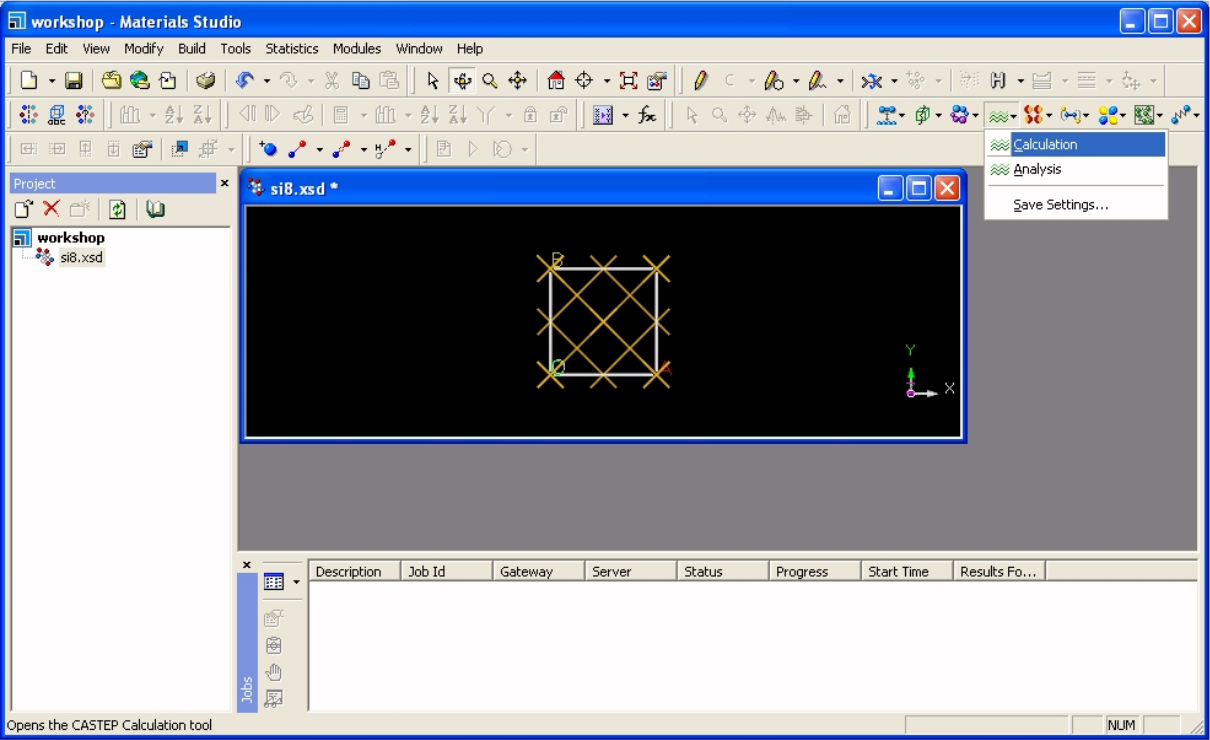
\includegraphics[height=2.62in,width=4.00in,viewport=0 0 1210 740,clip]{Figures/MS-CASTEP-01-Si.png}
\caption{\tiny \textrm{CASTEP Calculation by Materials studio:~Si.}}%(与文献\cite{EPJB33-47_2003}图1对比)
\label{MS-CASTEP-Calculation-01}
\end{figure}
}

\frame
{
	\frametitle{\textrm{MS:~CASTEP Calculation example:~Si}}
\begin{figure}[h!]
\centering
%\vspace*{-0.10in}
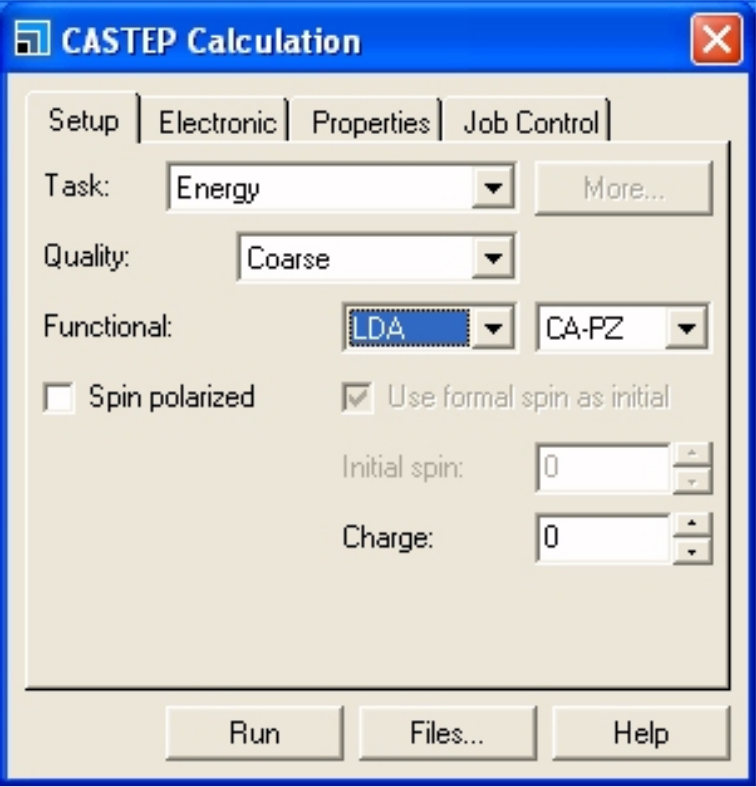
\includegraphics[height=2.05in,width=1.95in,viewport=0 0 756 787,clip]{Figures/MS-CASTEP-02-Si-parameter-1.png}
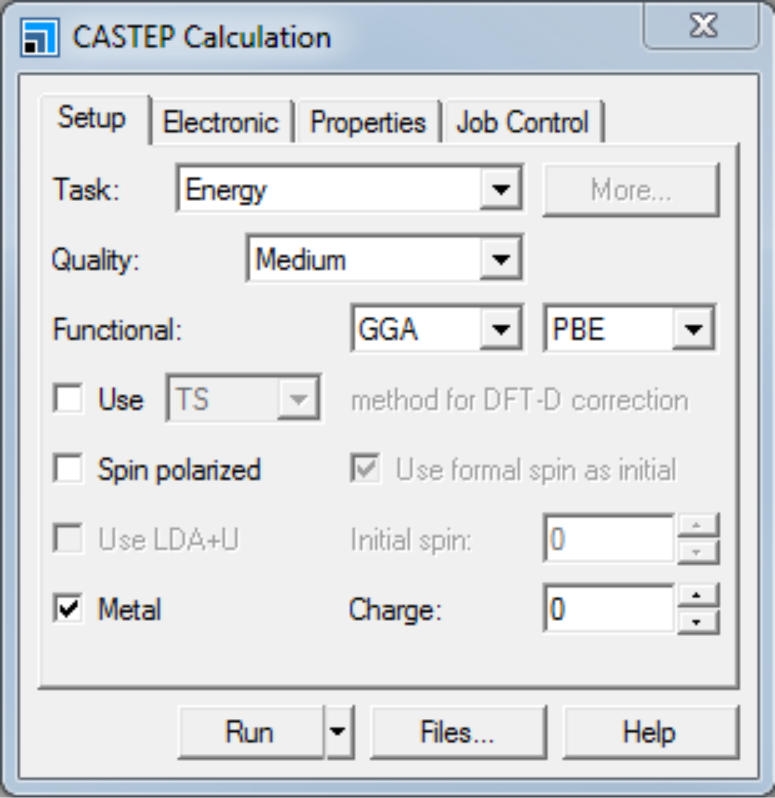
\includegraphics[height=2.05in,width=1.95in,viewport=0 0 775 798,clip]{Figures/MS-CASTEP-02-Si-parameter-2.png}
\caption{\tiny \textrm{CASTEP Calculation by Materials studio:~Parameter.}}%(与文献\cite{EPJB33-47_2003}图1对比)
\label{MS-CASTEP-Calculation-02}
\end{figure}
}

\frame
{
	\frametitle{\textrm{MS:~CASTEP Calculation example:~Si}}
\begin{figure}[h!]
\centering
\vspace*{-0.10in}
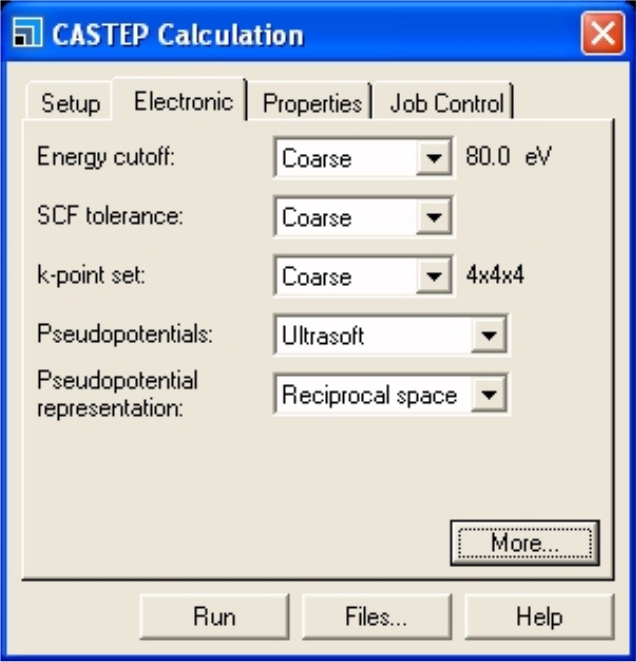
\includegraphics[height=2.15in,width=1.95in,viewport=0 -50 650 700,clip]{Figures/MS-CASTEP-13-Si-Calculat-Electron-step.png}
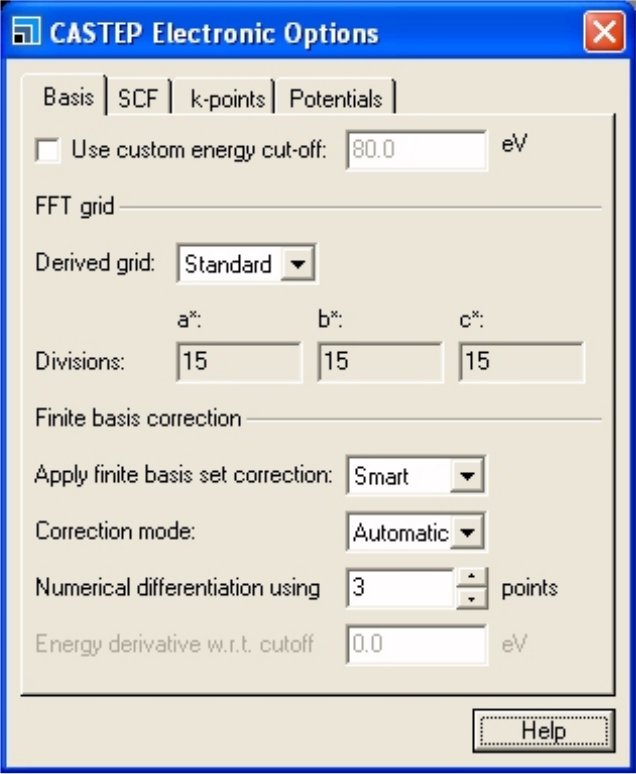
\includegraphics[height=2.15in,width=1.95in,viewport=0 0 636 774,clip]{Figures/MS-CASTEP-13-Si-Calculat-Electron-detail.png}
\caption{\tiny \textrm{CASTEP Calculation by Materials studio:~Electron-step.}}%(与文献\cite{EPJB33-47_2003}图1对比)
\label{MS-CASTEP-Calculation-electron}
\end{figure}
}

\frame
{
	\frametitle{\textrm{MS:~CASTEP Calculation example:~Si}}
\begin{figure}[h!]
\centering
%\vspace*{-0.10in}
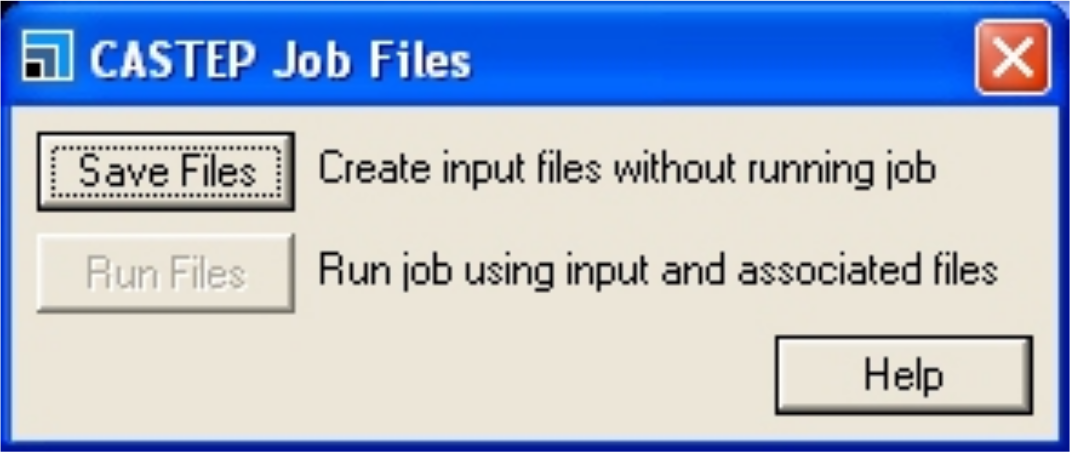
\includegraphics[height=1.15in,width=3.30in,viewport=0 0 1070 452,clip]{Figures/MS-CASTEP-03-Si-input-1.png}
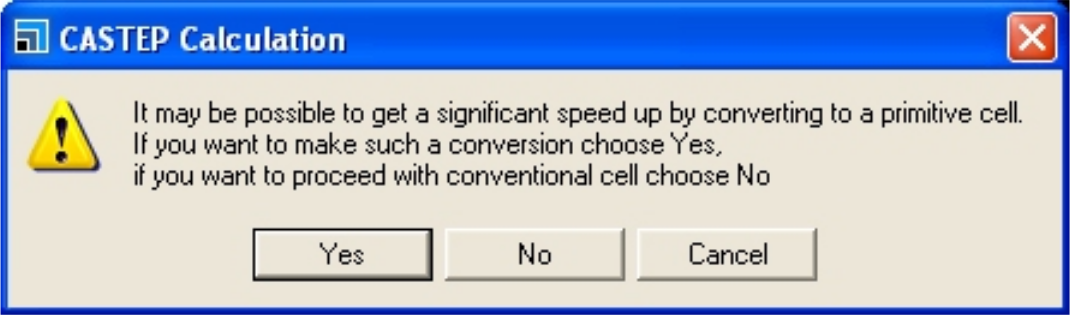
\includegraphics[height=1.15in,width=4.00in,viewport=0 0 1070 355,clip]{Figures/MS-CASTEP-03-Si-input-2.png}
\caption{\tiny \textrm{CASTEP Calculation.}}%(与文献\cite{EPJB33-47_2003}图1对比)
\label{MS-CASTEP-Calculation-03}
\end{figure}
}

\frame
{
	\frametitle{\textrm{MS:~CASTEP Calculation example:~Si}}
\begin{figure}[h!]
\centering
\vspace*{-0.10in}
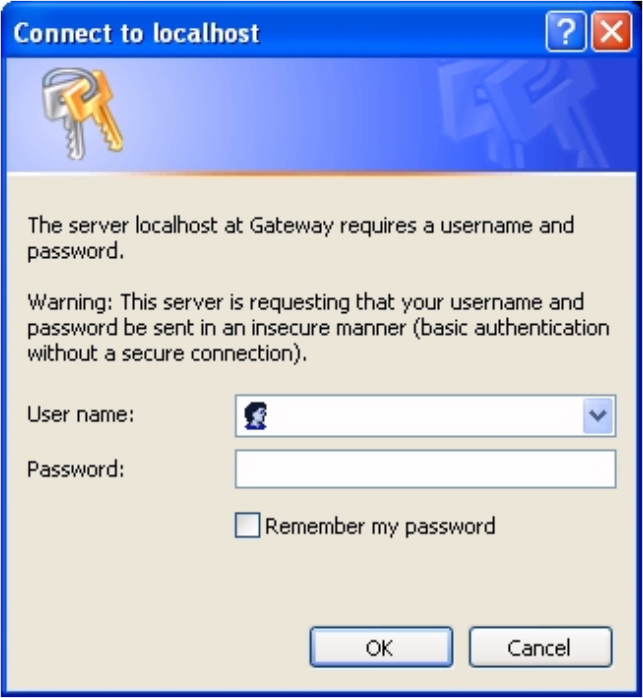
\includegraphics[height=2.65in,width=2.63in,viewport=0 0 643 698,clip]{Figures/MS-CASTEP-04-Si-sever.png}
\caption{\tiny \textrm{CASTEP Calculation by Materials studio:~Connect to localhost.}}%(与文献\cite{EPJB33-47_2003}图1对比)
\label{MS-CASTEP-Calculation-sever}
\end{figure}
}

\frame
{
	\frametitle{\textrm{MS:~CASTEP Calculation example:~Si}}
\begin{figure}[h!]
\centering
\vspace*{-0.10in}
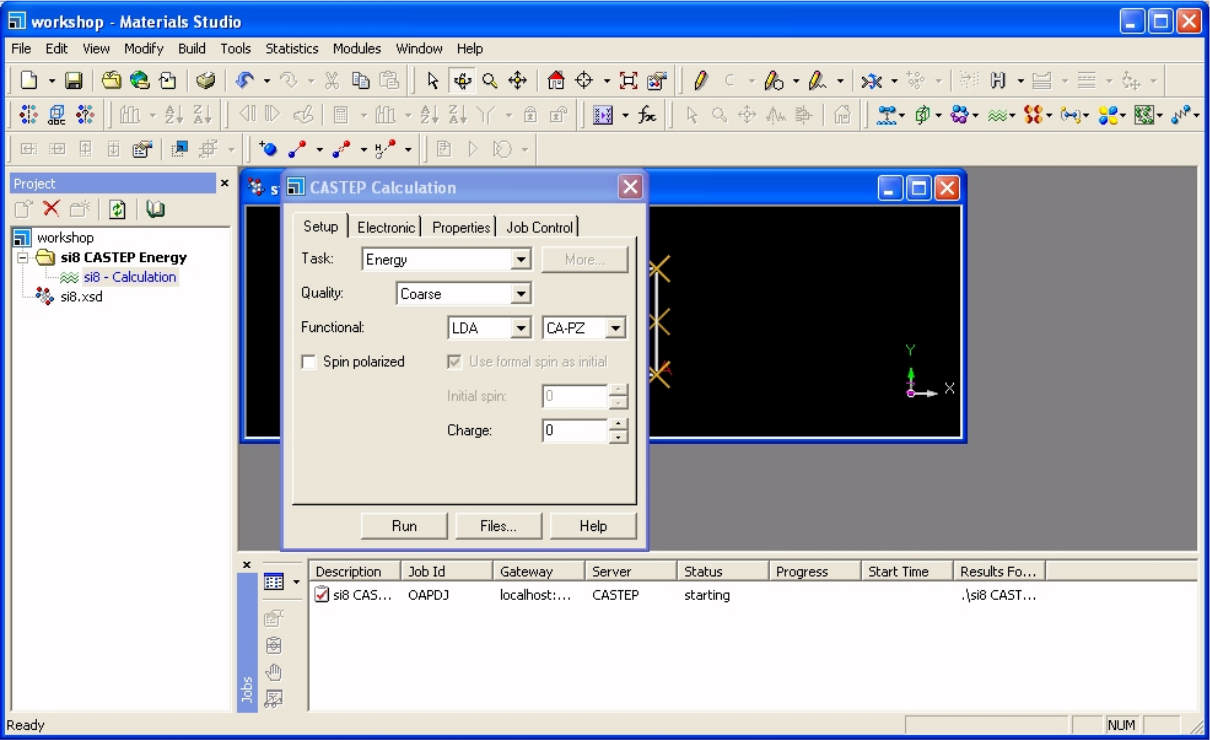
\includegraphics[height=2.60in,width=4.00in,viewport=0 0 1210 740,clip]{Figures/MS-CASTEP-05-Si-Calculat.png}
\caption{\tiny \textrm{CASTEP Calculation by Materials studio:~Run.}}%(与文献\cite{EPJB33-47_2003}图1对比)
\label{MS-CASTEP-Calculation-Run}
\end{figure}
}

\frame
{
	\frametitle{\textrm{MS:~CASTEP Calculation example:~Si}}
\begin{figure}[h!]
\centering
%\vspace*{-0.10in}
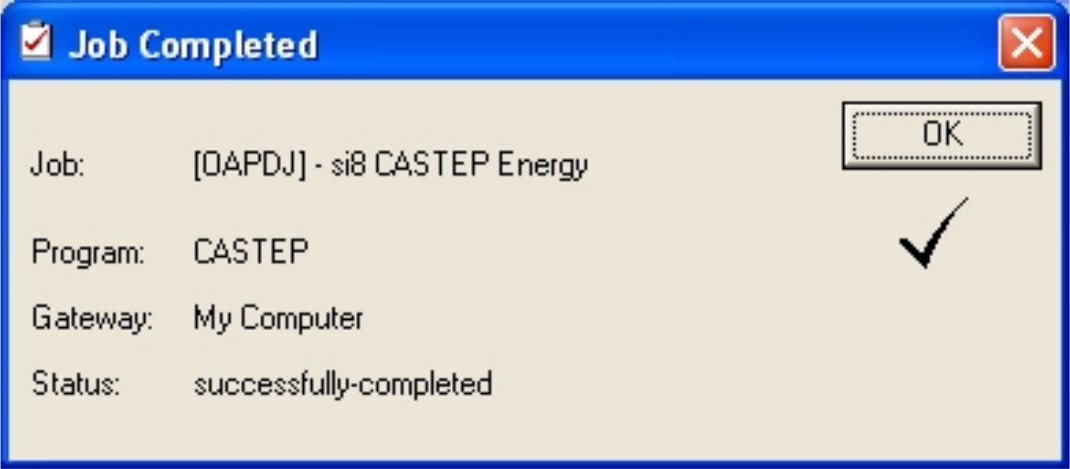
\includegraphics[height=1.50in,width=4.00in,viewport=0 0 1070 469,clip]{Figures/MS-CASTEP-06-Si-Calculat-finish.png}
\caption{\tiny \textrm{CASTEP Calculation by Materials studio:~Complete.}}%(与文献\cite{EPJB33-47_2003}图1对比)
\label{MS-CASTEP-Calculation-Complete}
\end{figure}
}

\frame
{
	\frametitle{\textrm{MS:~CASTEP Calculation example:~Si}}
\begin{figure}[h!]
\centering
\vspace*{-0.10in}
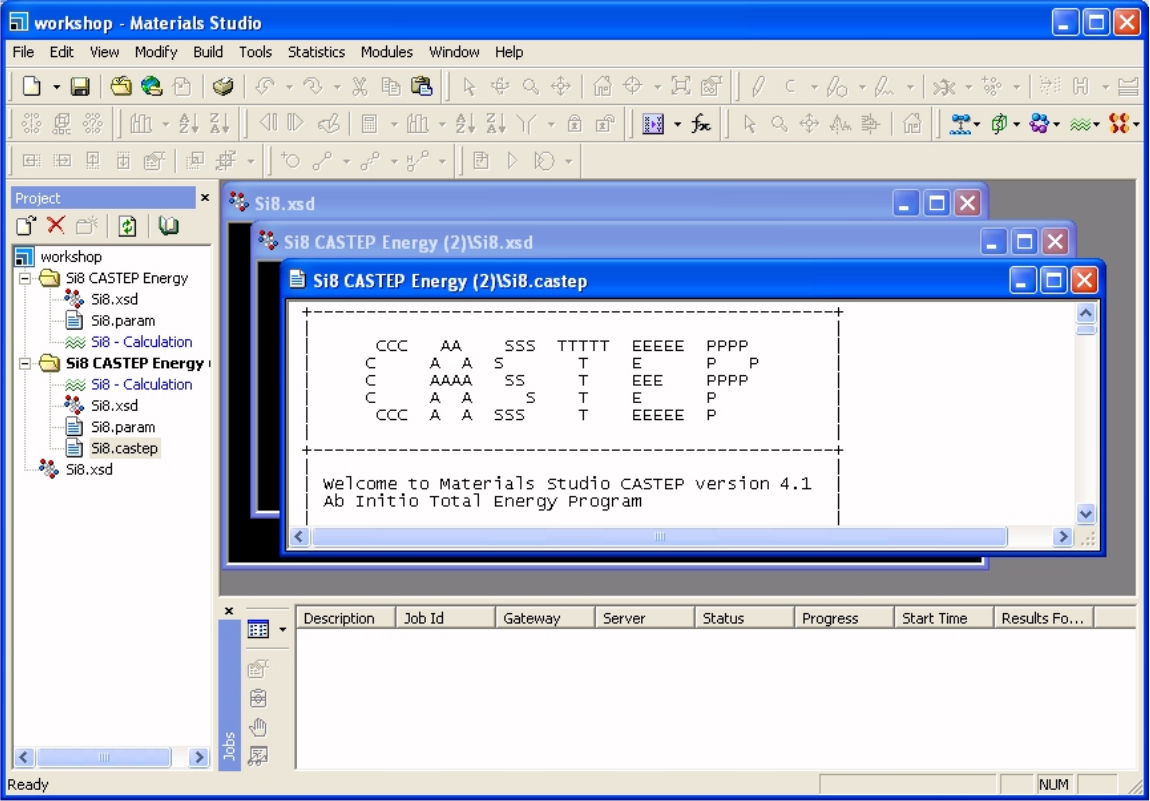
\includegraphics[height=2.66in,width=4.00in,viewport=0 0 1150 801,clip]{Figures/MS-CASTEP-07-Si-Calculat-data.png}
\caption{\tiny \textrm{CASTEP Calculation by Materials studio:~Finish.}}%(与文献\cite{EPJB33-47_2003}图1对比)
\label{MS-CASTEP-Calculation-data}
\end{figure}
}

\frame
{
	\frametitle{\textrm{MS:~CASTEP Calculation example:~Si}}
\begin{figure}[h!]
\centering
\vspace*{-0.10in}
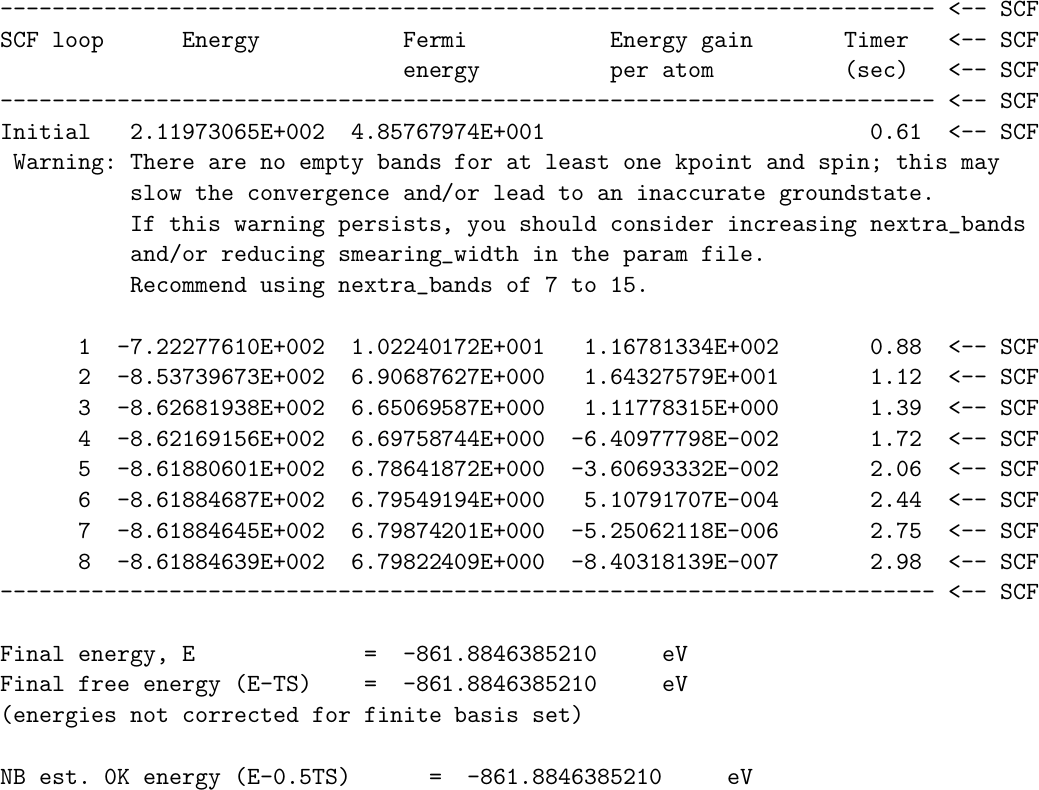
\includegraphics[height=2.60in,width=4.00in,viewport=0 0 1039 790,clip]{Figures/MS-CASTEP-08-Si-Calculat-SCF.png}
\caption{\tiny \textrm{CASTEP Calculation by Materials studio:~SCF.}}%(与文献\cite{EPJB33-47_2003}图1对比)
\label{MS-CASTEP-Calculation-SCF}
\end{figure}
}

\frame
{
	\frametitle{\textrm{MS:~CASTEP Analysis example:~Si}}
\begin{figure}[h!]
\centering
\vspace*{-0.10in}
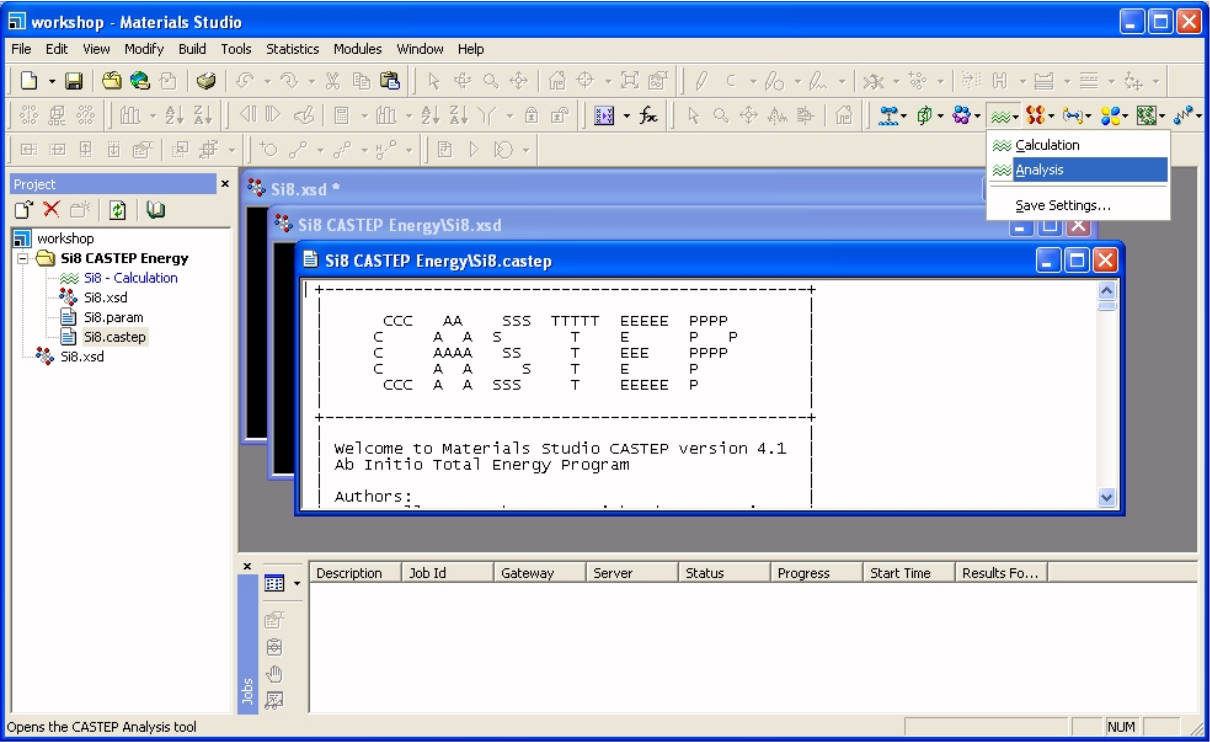
\includegraphics[height=2.60in,width=4.00in,viewport=0 0 1210 742,clip]{Figures/MS-CASTEP-09-Si-Analysis.png}
\caption{\tiny \textrm{CASTEP Analysis by Materials studio.}}%(与文献\cite{EPJB33-47_2003}图1对比)
\label{MS-CASTEP-Analysis}
\end{figure}
}

\frame
{
	\frametitle{\textrm{MS:~CASTEP Analysis example:~Si}}
\begin{figure}[h!]
\centering
\vspace*{-0.10in}
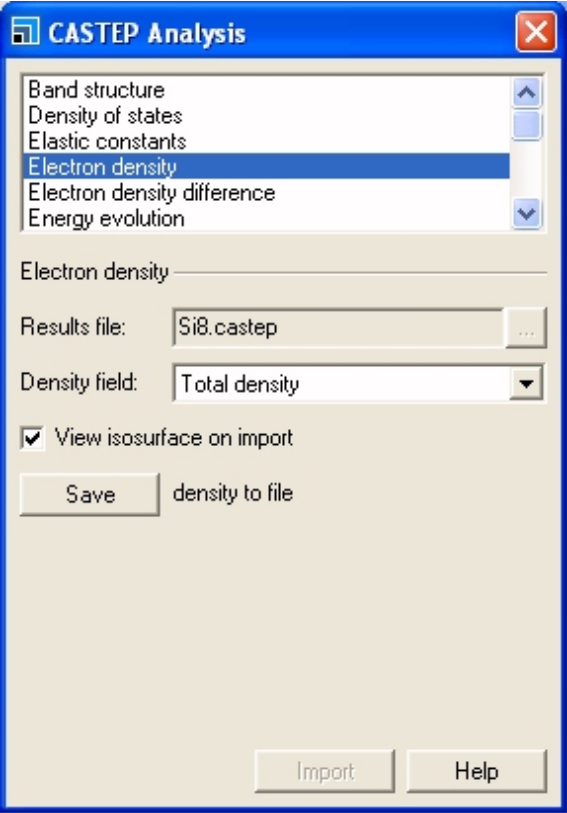
\includegraphics[height=2.66in,width=2.30in,viewport=0 0 567 813,clip]{Figures/MS-CASTEP-10-Si-Analysis-parameter.png}
\caption{\tiny \textrm{CASTEP Analysis by Materials studio:~Parameter.}}%(与文献\cite{EPJB33-47_2003}图1对比)
\label{MS-CASTEP-Analysis-parameter}
\end{figure}
}

\frame
{
	\frametitle{\textrm{MS:~CASTEP Analysis example:~Si}}
\begin{figure}[h!]
\centering
\vspace*{-0.10in}
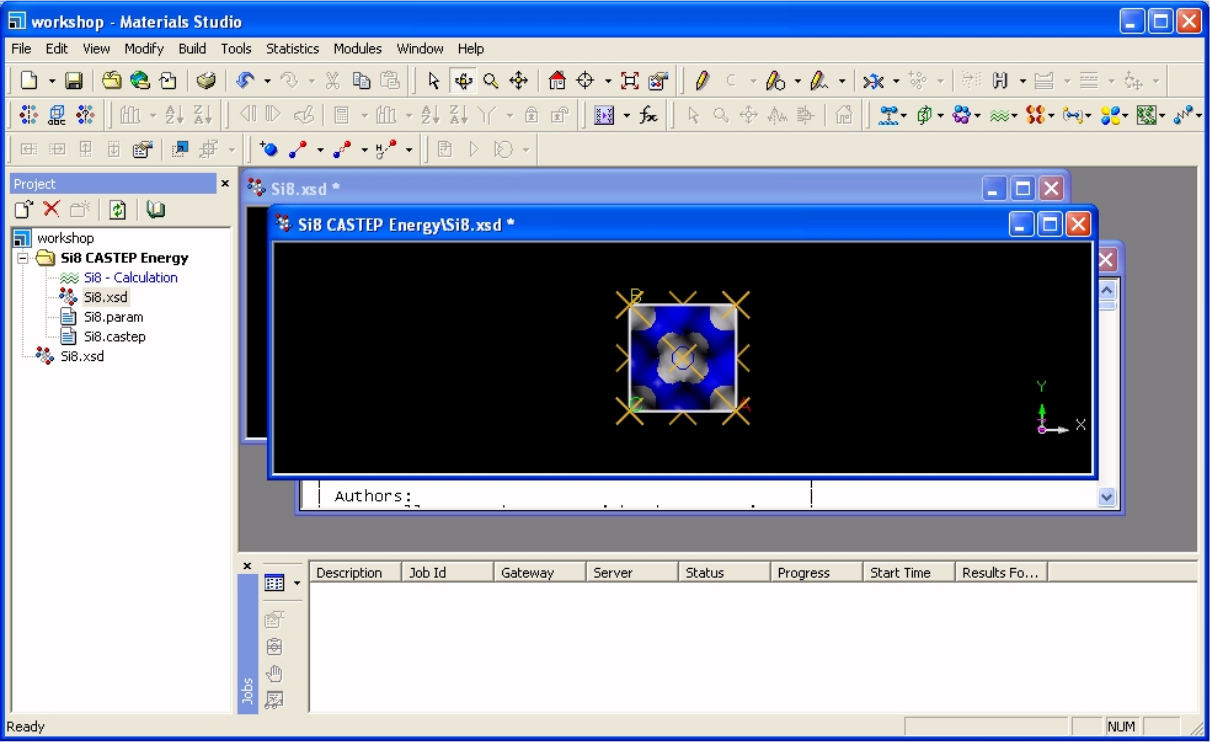
\includegraphics[height=2.60in,width=4.00in,viewport=0 0 1210 742,clip]{Figures/MS-CASTEP-11-Si-Analysis-charge.png}
\caption{\tiny \textrm{CASTEP Analysis by Materials studio:~Charge.}}%(与文献\cite{EPJB33-47_2003}图1对比)
\label{MS-CASTEP-Analysis-Charge}
\end{figure}
}

\frame
{
	\frametitle{\textrm{MS:~CASTEP Analysis example:~Si}}
\begin{figure}[h!]
\centering
\vspace*{-0.10in}
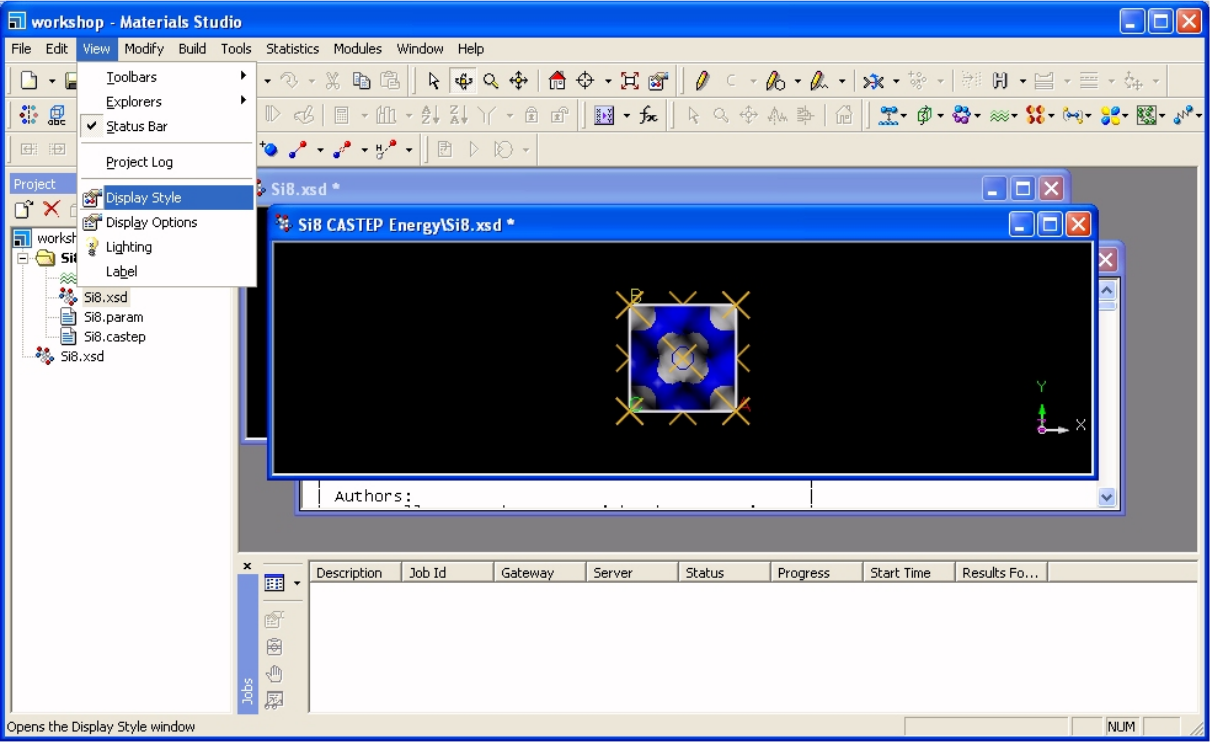
\includegraphics[height=2.60in,width=4.00in,viewport=0 0 1210 742,clip]{Figures/MS-CASTEP-11-Si-Analysis-display.png}
\caption{\tiny \textrm{CASTEP Analysis by Materials studio:~Display-style.}}%(与文献\cite{EPJB33-47_2003}图1对比)
\label{MS-CASTEP-Analysis-display}
\end{figure}
}

\frame
{
	\frametitle{\textrm{MS:~CASTEP Analysis example:~Si}}
\begin{figure}[h!]
\centering
%\vspace*{-0.10in}
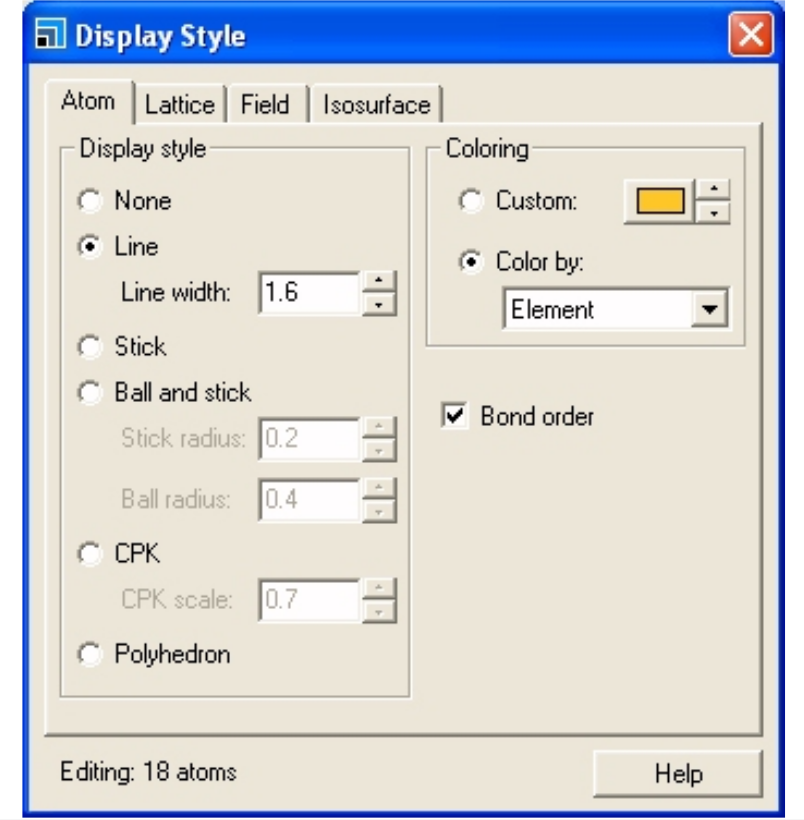
\includegraphics[height=2.00in,width=1.95in,viewport=0 0 810 820,clip]{Figures/MS-CASTEP-12-Si-Analysis-display-parameter-1.png}
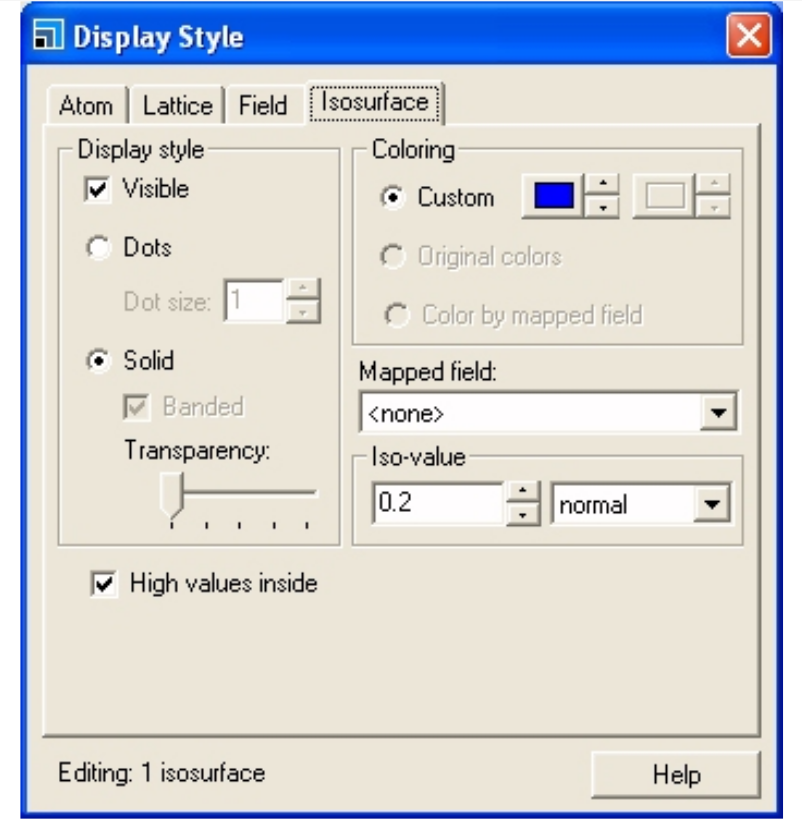
\includegraphics[height=2.00in,width=1.95in,viewport=0 0 802 822,clip]{Figures/MS-CASTEP-12-Si-Analysis-display-parameter-2.png}
\caption{\tiny \textrm{CASTEP Analysis by Materials studio:~Display-parameter.}}%(与文献\cite{EPJB33-47_2003}图1对比)
\label{MS-CASTEP-Analysis-display-parameter}
\end{figure}
}

\frame
{
	\frametitle{\textrm{MS:~CASTEP Analysis example:~Si}}
\begin{figure}[h!]
\centering
%\vspace*{-0.10in}
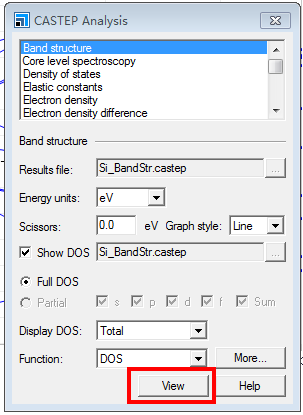
\includegraphics[height=2.60in,width=2.20in,viewport=4 0 300 415,clip]{Figures/MS-CASTEP-14-Si-Analysis-Band_DOS-parameter.png}
\caption{\tiny \textrm{CASTEP Analysis by Materials studio:~Display Band and DOS parameter.}}%(与文献\cite{EPJB33-47_2003}图1对比)
\label{MS-CASTEP-Analysis-display-Band_DOS-parameter}
\end{figure}
}

\frame
{
	\frametitle{\textrm{MS:~CASTEP Analysis example:~Si}}
\begin{figure}[h!]
\centering
%\vspace*{-0.10in}
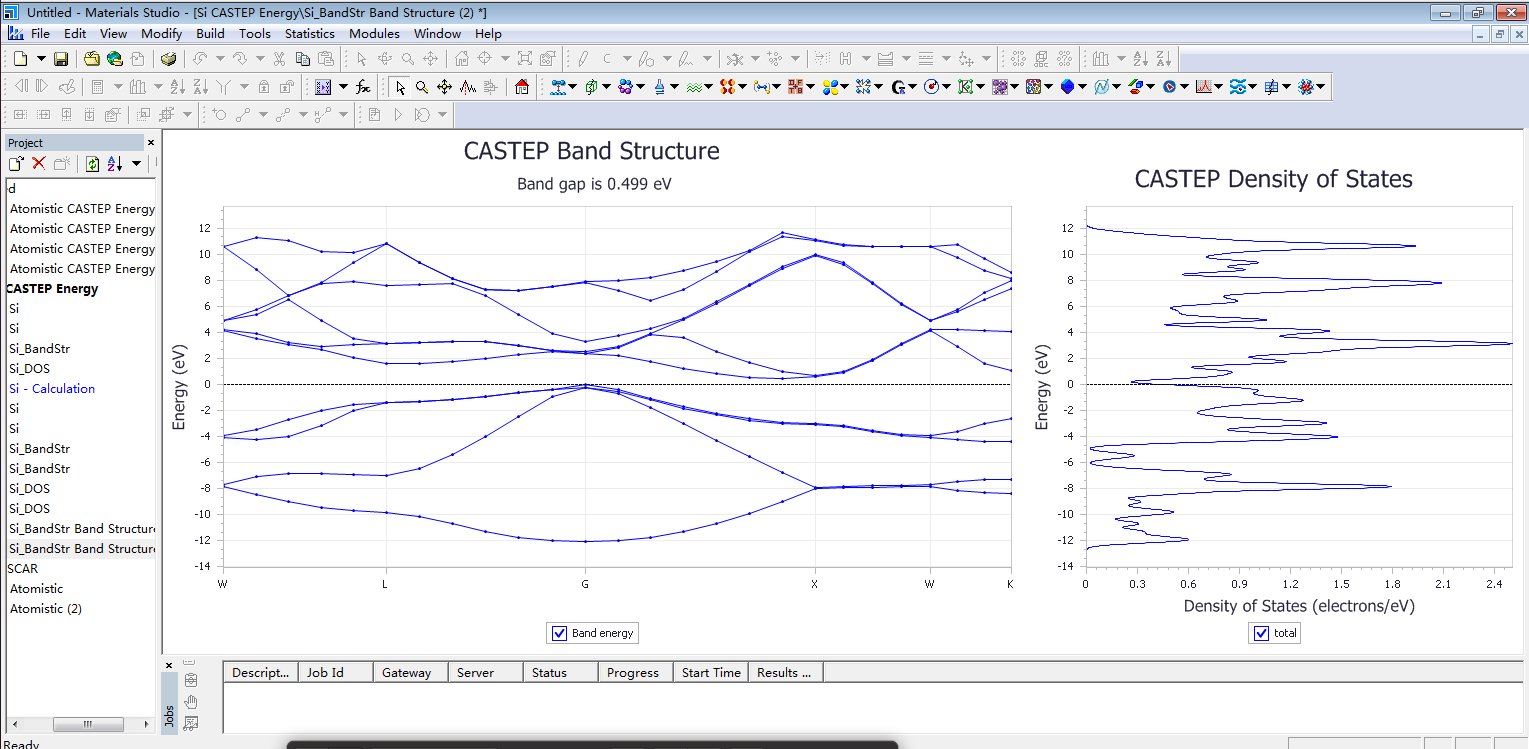
\includegraphics[height=2.00in,width=4.05in,viewport=0 0 1529 749,clip]{Figures/MS-CASTEP-14-Si-Analysis-Band_DOS.png}
\caption{\tiny \textrm{CASTEP Analysis by Materials studio:~Display Band and DOS.}}%(与文献\cite{EPJB33-47_2003}图1对比)
\label{MS-CASTEP-Analysis-display-Band_DOS}
\end{figure}
}

\frame
{
	\frametitle{\textrm{MS:~MD Calculation:~Dynamics}}
\begin{figure}[h!]
\centering
%\vspace*{-0.10in}
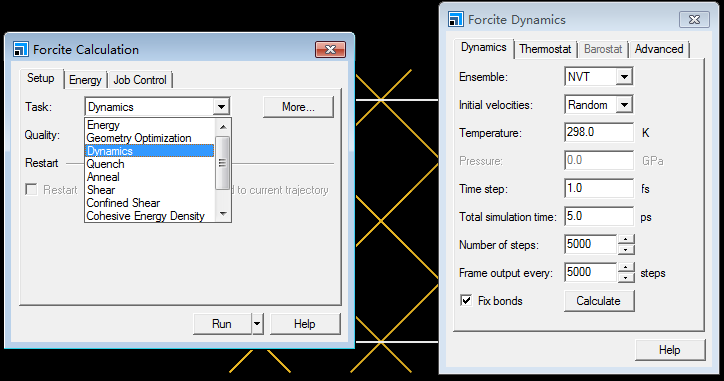
\includegraphics[height=2.10in,width=4.05in,viewport=0 0 724 381,clip]{Figures/MS-MD-Dynamics.png}
\caption{\tiny \textrm{MD Calculation by Materials studio.}}%(与文献\cite{EPJB33-47_2003}图1对比)
\label{MS-MD-Dynamics}
\end{figure}
}

\frame
{
	\frametitle{\textrm{MS:~MD Calculation:~Ensemble}}
\begin{figure}[h!]
\centering
%\vspace*{-0.10in}
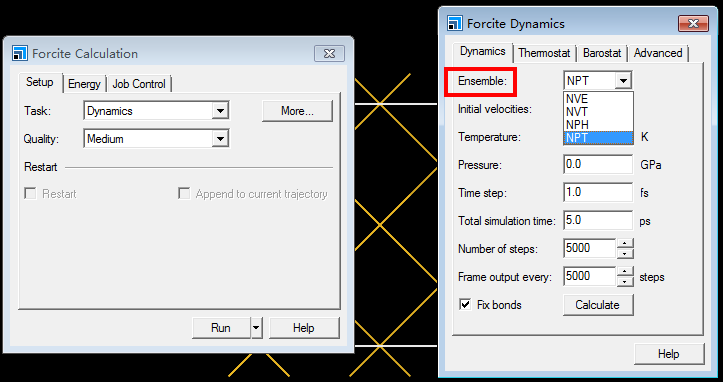
\includegraphics[height=2.10in,width=4.05in,viewport=0 0 723 382,clip]{Figures/MS-MD-ensemble.png}
\caption{\tiny \textrm{MD Calculation by Materials studio:~Ensemble.}}%(与文献\cite{EPJB33-47_2003}图1对比)
\label{MS-MD-Dynamics-Ensemble}
\end{figure}
}

\frame
{
	\frametitle{\textrm{MS:~MD Calculation:~Themostat}}
\begin{figure}[h!]
\centering
%\vspace*{-0.10in}
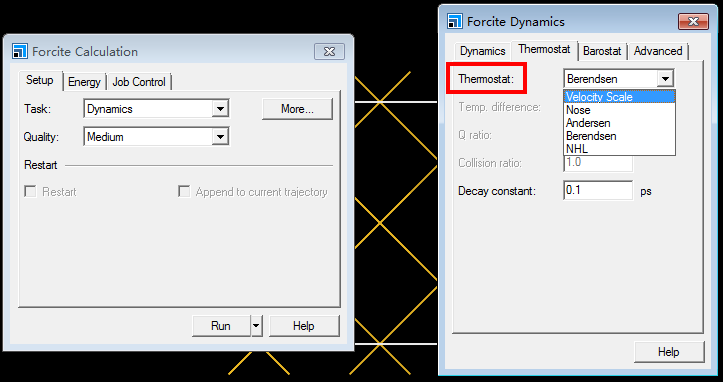
\includegraphics[height=2.10in,width=4.05in,viewport=0 0 723 382,clip]{Figures/MS-MD-Themostat.png}
\caption{\tiny \textrm{MD Calculation by Materials studio:~Themostat.}}%(与文献\cite{EPJB33-47_2003}图1对比)
\label{MS-MD-Dynamics-Themostat}
\end{figure}
}

\frame
{
	\frametitle{\textrm{MS:~MD Calculation:~Barostat}}
\begin{figure}[h!]
\centering
%\vspace*{-0.10in}
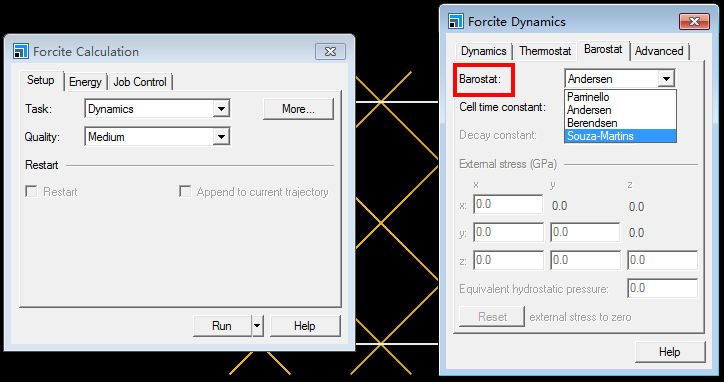
\includegraphics[height=2.10in,width=4.05in,viewport=0 0 724 382,clip]{Figures/MS-MD-Barostat.png}
\caption{\tiny \textrm{MD Calculation by Materials studio:~Barostat.}}%(与文献\cite{EPJB33-47_2003}图1对比)
\label{MS-MD-Dynamics-Barostat}
\end{figure}
}

\frame
{
	\frametitle{\textrm{MS:~MD Calculation:~Force-Field}}
\begin{figure}[h!]
\centering
%\vspace*{-0.10in}
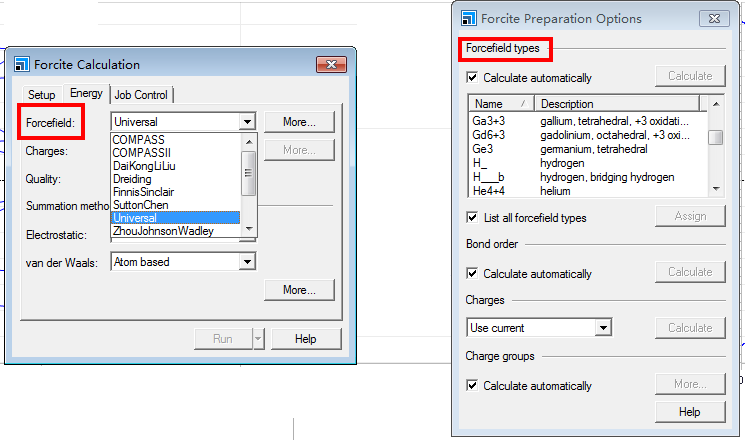
\includegraphics[height=2.40in,width=4.05in,viewport=0 0 745 440,clip]{Figures/MS-MD-Force-Field.png}
\caption{\tiny \textrm{MD Calculation by Materials studio:~Force-Field.}}%(与文献\cite{EPJB33-47_2003}图1对比)
\label{MS-MD-Dynamics-ForceField}
\end{figure}
}

\frame
{
	\frametitle{\textrm{MS:~MD Calculation:~Electrostatic}}
\begin{figure}[h!]
\centering
%\vspace*{-0.10in}
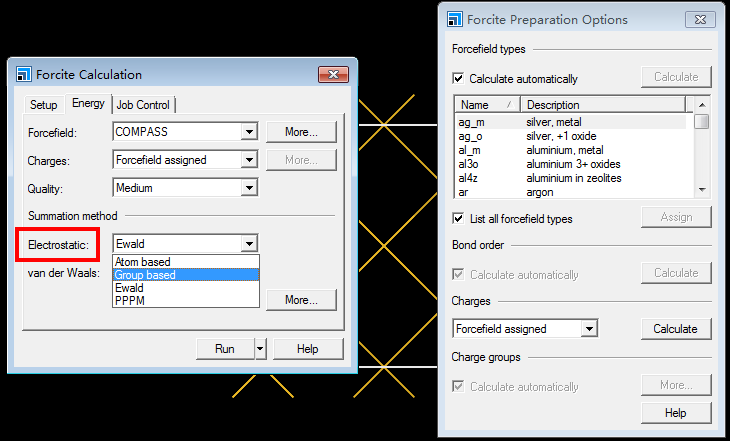
\includegraphics[height=2.40in,width=4.05in,viewport=0 0 730 441,clip]{Figures/MS-MD-Electrostatic.png}
\caption{\tiny \textrm{MD Calculation by Materials studio:~Electrostatic.}}%(与文献\cite{EPJB33-47_2003}图1对比)
\label{MS-MD-Dynamics-Electrostatic}
\end{figure}
}

\section{\rm{Materials~Studio}建模}
\frame
{
	\frametitle{\textrm{MS~Modelling:~Polymers}}
\begin{figure}[h!]
\centering
\vspace*{-0.05in}
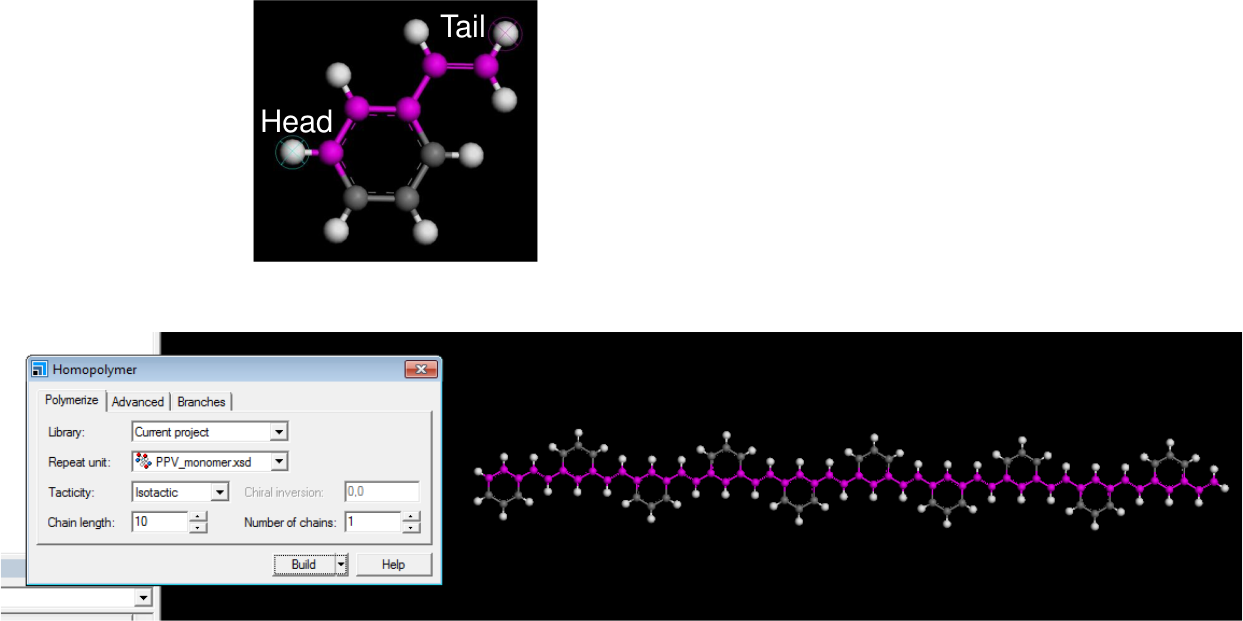
\includegraphics[height=2.10in,width=4.00in,viewport=0 0 1280 650,clip]{Figures/MS-Building_homopolymer.png}
\caption{\tiny \textrm{Building homopolymer for Materials studio.}}%(与文献\cite{EPJB33-47_2003}图1对比)
\label{MS-Building_homopolymer}
\end{figure}
}

\frame
{
	\frametitle{\textrm{MS~Modelling:~Polymers}}
\begin{figure}[h!]
\centering
\vspace*{-0.05in}
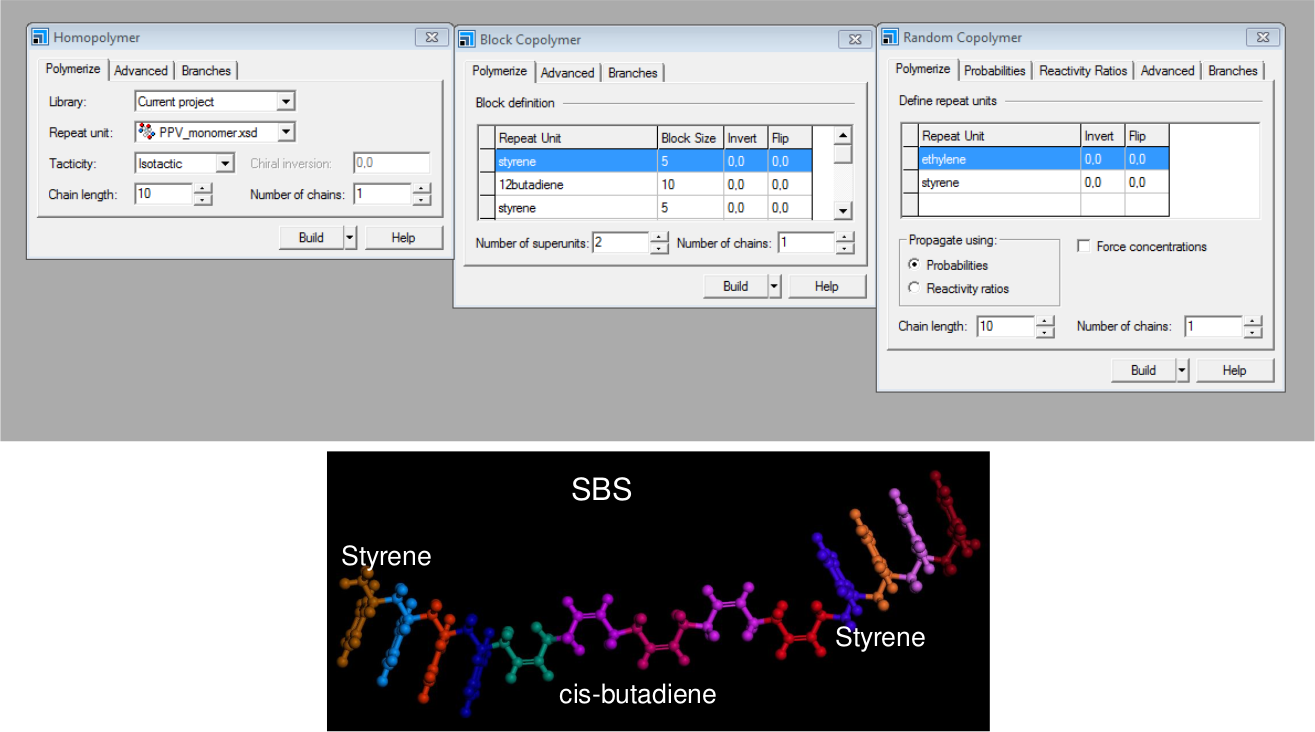
\includegraphics[height=2.20in,width=4.00in,viewport=0 0 1350 740,clip]{Figures/MS-Building_multypolymer.png}
\caption{\tiny \textrm{Building multi-polymer for Materials studio.}}%(与文献\cite{EPJB33-47_2003}图1对比)
\label{MS-Building_multypolymer}
\end{figure}
}

\frame
{
	\frametitle{\textrm{MS~Modelling:~amidoamine}}
\begin{figure}[h!]
\centering
\vspace*{-0.10in}
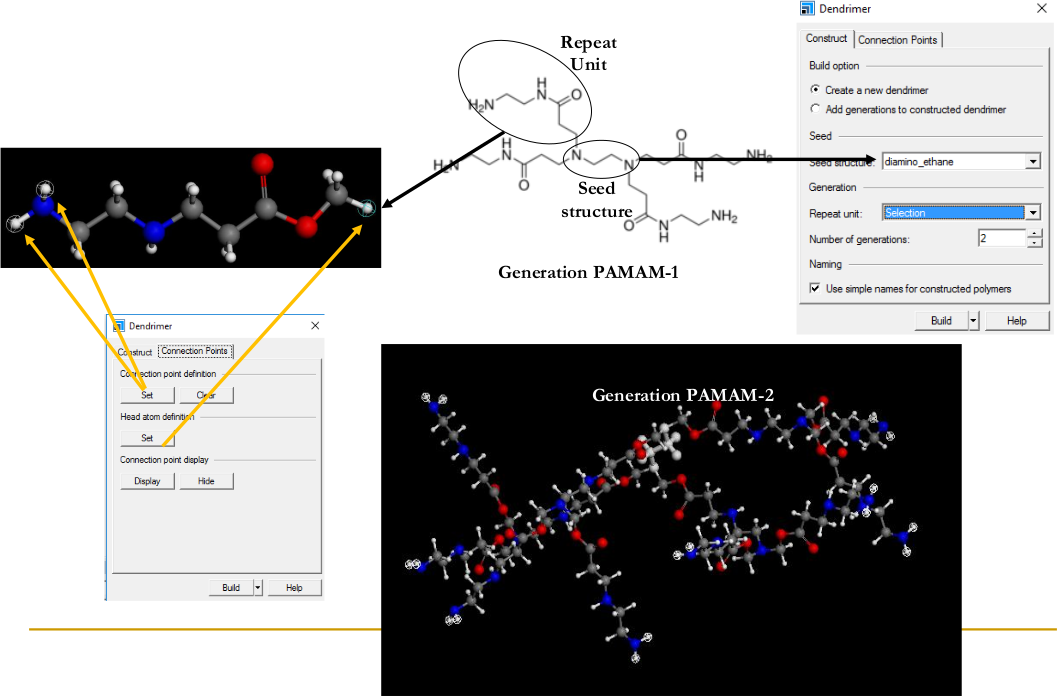
\includegraphics[height=2.45in,width=4.00in,viewport=0 0 1050 700,clip]{Figures/MS-Building_dendrimer.png}
\caption{\tiny \textrm{Building Poly-amidoamine (PAMAM) for Materials studio.}}%(与文献\cite{EPJB33-47_2003}图1对比)
\label{MS-Building_dendrimer}
\end{figure}
}

\frame
{
	\frametitle{\textrm{MS~Modelling:~from similar}}
\begin{figure}[h!]
\centering
\vspace*{-0.16in}
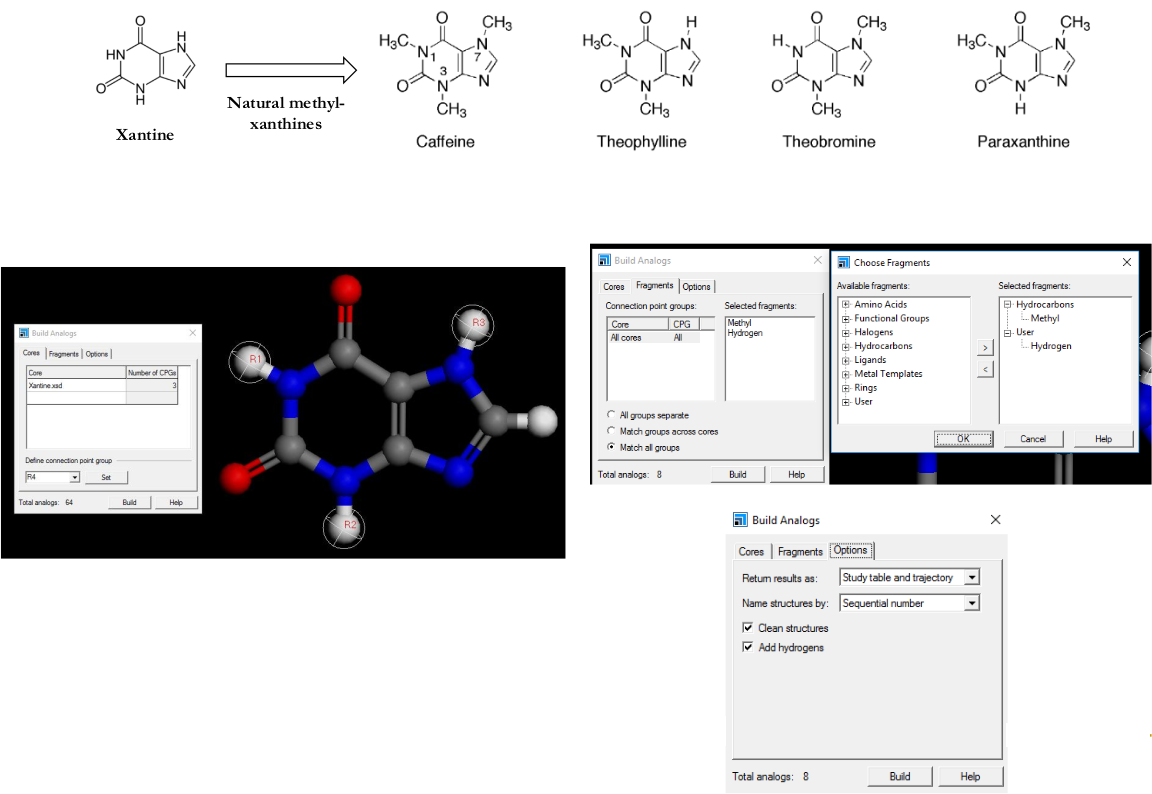
\includegraphics[height=2.65in,width=4.00in,viewport=0 0 1150 800,clip]{Figures/MS-Building_Analogs.png}
\caption{\tiny \textrm{Building from similar structure for Materials studio.}}%(与文献\cite{EPJB33-47_2003}图1对比)
\label{MS-Building_analogs}
\end{figure}
}

\frame
{
	\frametitle{\textrm{MS~Modelling:~from similar}}
\begin{figure}[h!]
\centering
%\vspace*{-0.10in}
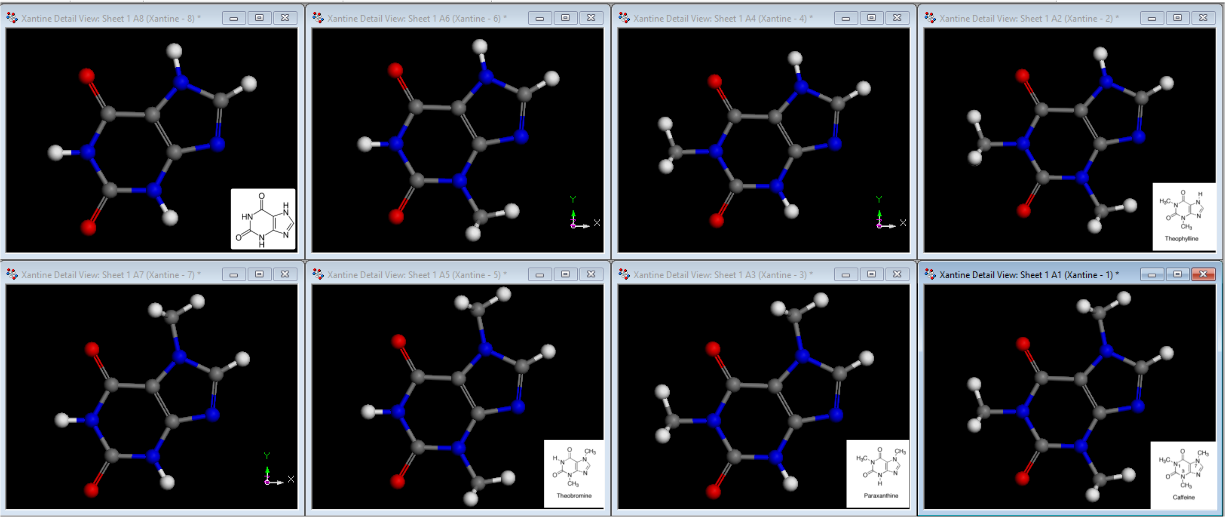
\includegraphics[height=1.70in,width=4.00in,viewport=0 0 1225 517,clip]{Figures/MS-Building_Analogs-examples.png}
\caption{\tiny \textrm{The similar structures in Materials studio.}}%(与文献\cite{EPJB33-47_2003}图1对比)
\label{MS-Building_analogs-examples}
\end{figure}
}

\frame
{
	\frametitle{\textrm{MS~Modelling:~Single-wall Nanotubes}}
\begin{figure}[h!]
\centering
\vspace*{-0.16in}
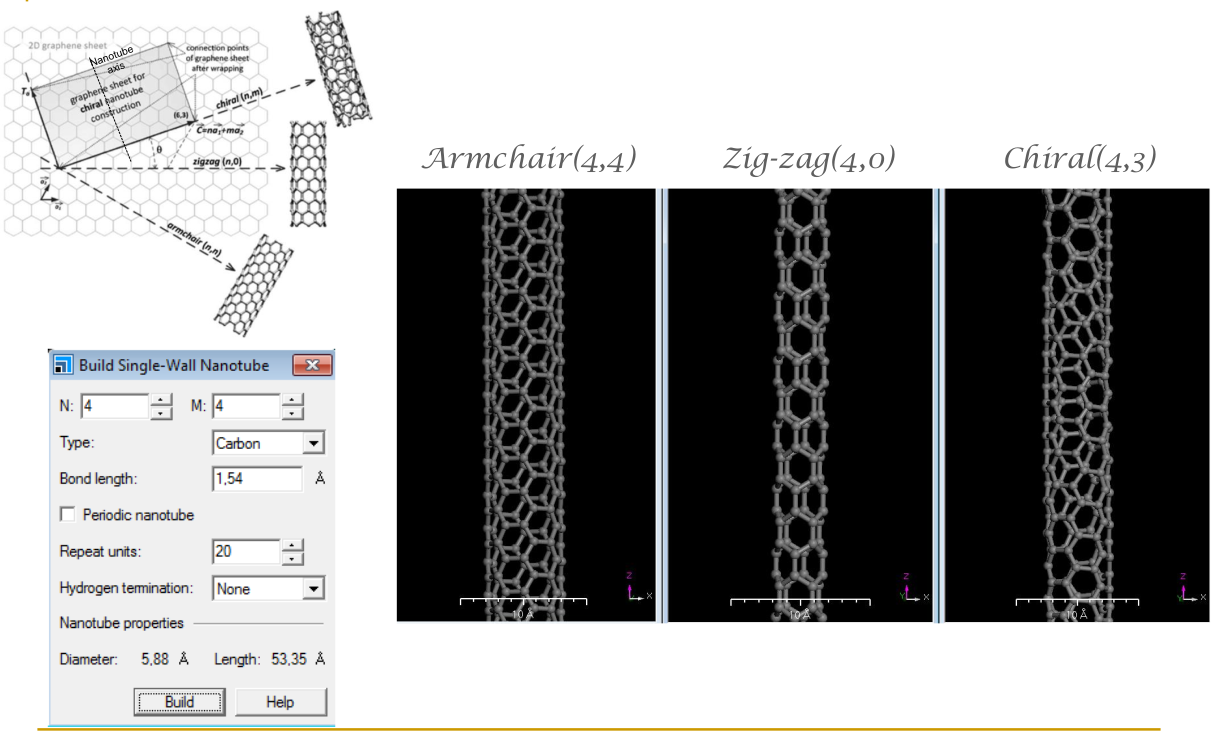
\includegraphics[height=2.60in,width=4.00in,viewport=0 0 1211 731,clip]{Figures/MS-Building_Single_wall-nanotube.png}
\caption{\tiny \textrm{Building Single-wall Nanotubes for Materials studio.}}%(与文献\cite{EPJB33-47_2003}图1对比)
\label{MS-Building_Single_wall-Nanotubes}
\end{figure}
}

\frame
{
	\frametitle{\textrm{MS~Modelling:~Single-wall Nanotubes}}
\begin{figure}[h!]
\centering
%\vspace*{-0.00in}
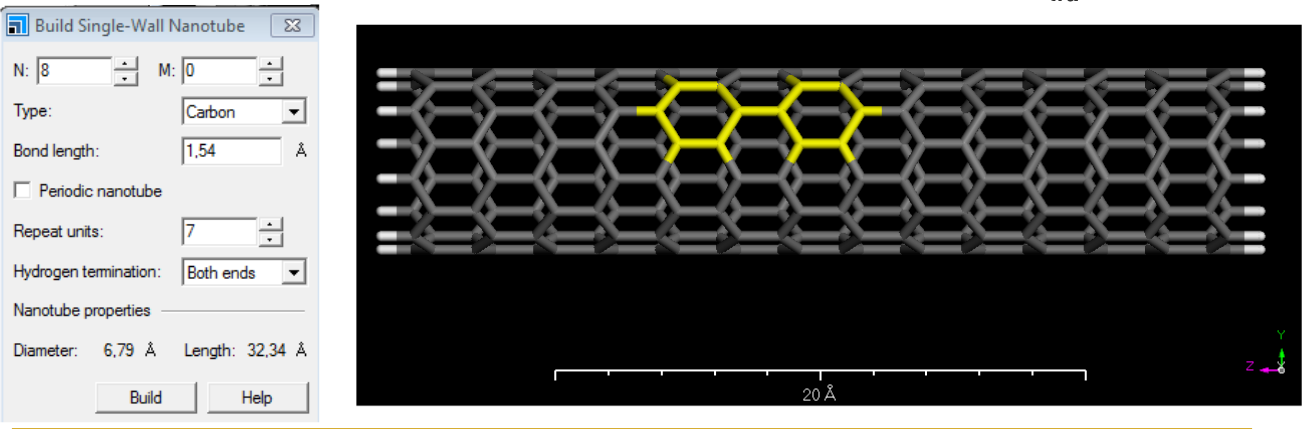
\includegraphics[height=1.32in,width=4.00in,viewport=0 0 1302 429,clip]{Figures/MS-Building_Single_wall-nanotube-example.png}
\caption{\tiny \textrm{Building Single-wall Nanobubes:~Select atoms for Materials studio.}}%(与文献\cite{EPJB33-47_2003}图1对比)
\label{MS-Building_Single_wall-Nanotubes-example}
\end{figure}
}

\frame
{
	\frametitle{\textrm{MS~Modelling:~Multi-wall Nanotubes}}
\begin{figure}[h!]
\centering
\vspace*{-0.16in}
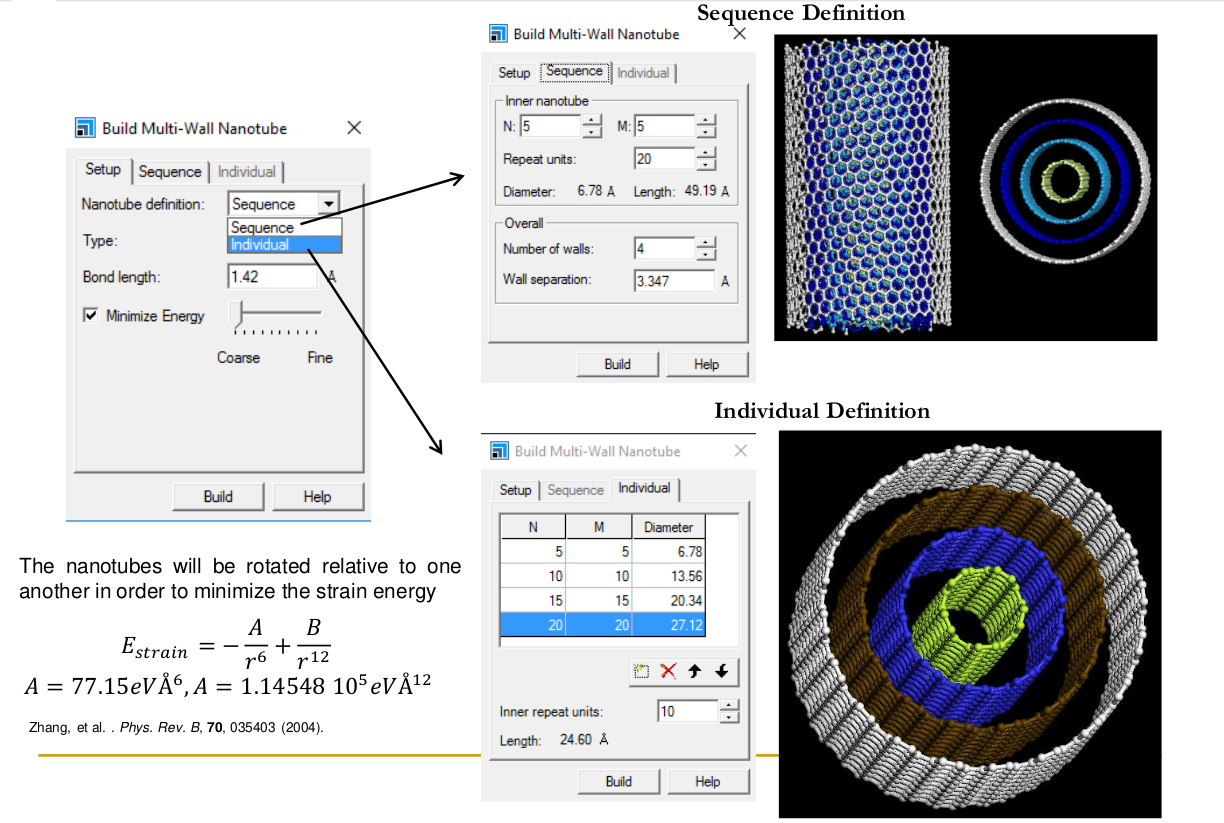
\includegraphics[height=2.68in,width=4.00in,viewport=0 0 1224 823,clip]{Figures/MS-Building_Multi_wall-nanotube.png}
\caption{\tiny \textrm{Building Multi-wall Nanotubes for Materials studio.}}%(与文献\cite{EPJB33-47_2003}图1对比)
\label{MS-Building_Multi_wall-Nanotubes}
\end{figure}
}

\frame
{
	\frametitle{\textrm{MS~Modelling:~Single-wall Nanotubes bundle}}
\begin{figure}[h!]
\centering
\vspace*{-0.18in}
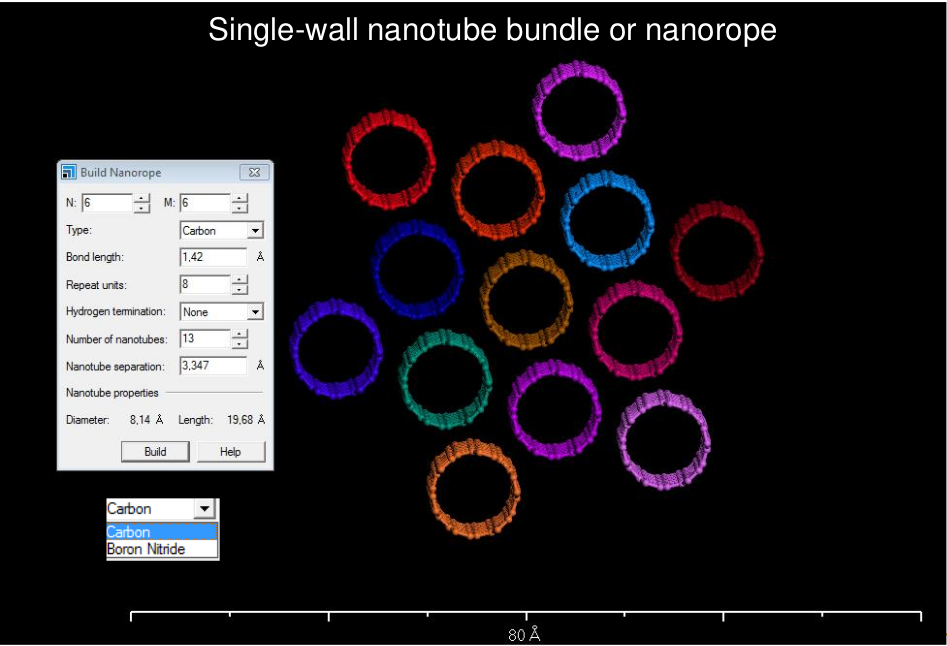
\includegraphics[height=2.70in,width=4.00in,viewport=0 0 947 646,clip]{Figures/MS-Building_Nanorope.png}
\caption{\tiny \textrm{Building Single-wall Nanotube bundle or nanorope for Materials studio.}}%(与文献\cite{EPJB33-47_2003}图1对比)
\label{MS-Building_Nanorope-bundle}
\end{figure}
}

\frame
{
	\frametitle{\textrm{MS~Modelling:~Construction of Nanocluster}}
\begin{figure}[h!]
\centering
\vspace*{-0.15in}
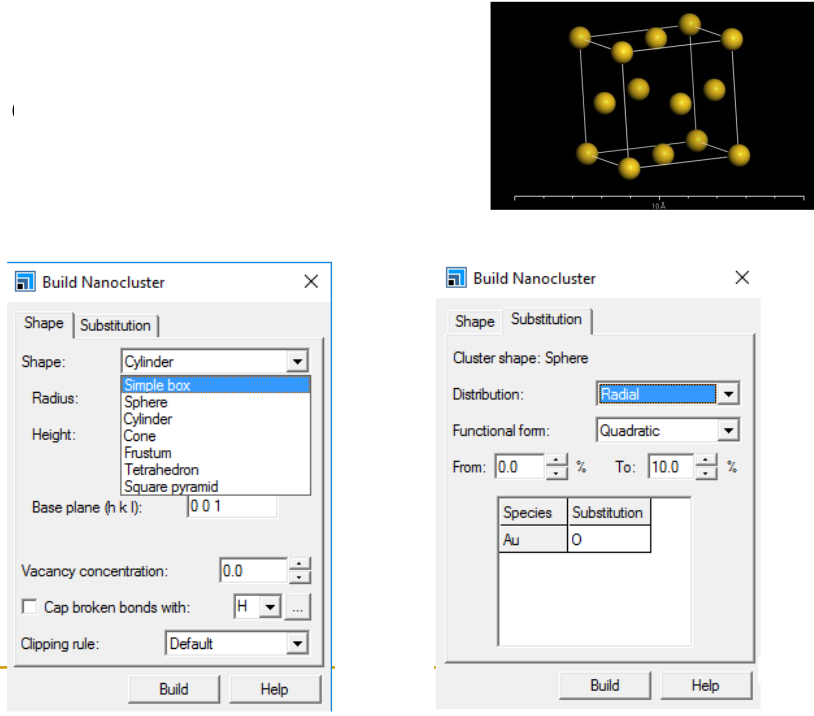
\includegraphics[height=2.45in,width=2.90in,viewport=0 0 814 716,clip]{Figures/MS-Building_Nanocluster.png}
\caption{\tiny \textrm{Building of Nanocluster for Materials studio.}}%(与文献\cite{EPJB33-47_2003}图1对比)
\label{MS-Building_Nanocluster}
\end{figure}
}

\frame
{
	\frametitle{\textrm{MS~Modelling:~Construction of Nanocluster}}
\begin{figure}[h!]
\centering
\vspace*{-0.10in}
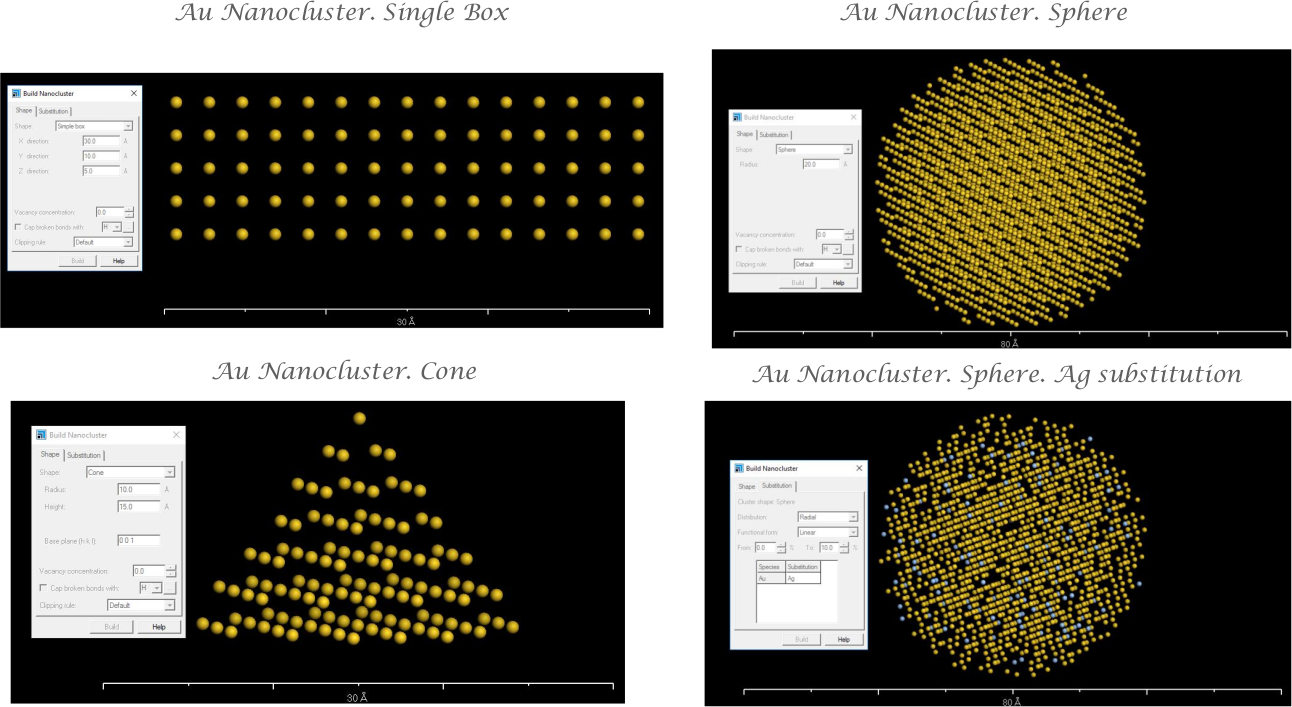
\includegraphics[height=2.20in,width=4.00in,viewport=0 0 1292 707,clip]{Figures/MS-Building_Nanocluster-examples.png}
\caption{\tiny \textrm{The Nanocluster structures in Materials studio.}}%(与文献\cite{EPJB33-47_2003}图1对比)
\label{MS-Building_Nanocluster-examples}
\end{figure}
}

\frame
{
	\frametitle{\textrm{MS~Modelling:~Meso-molecules}}
\begin{figure}[h!]
\centering
\vspace*{-0.12in}
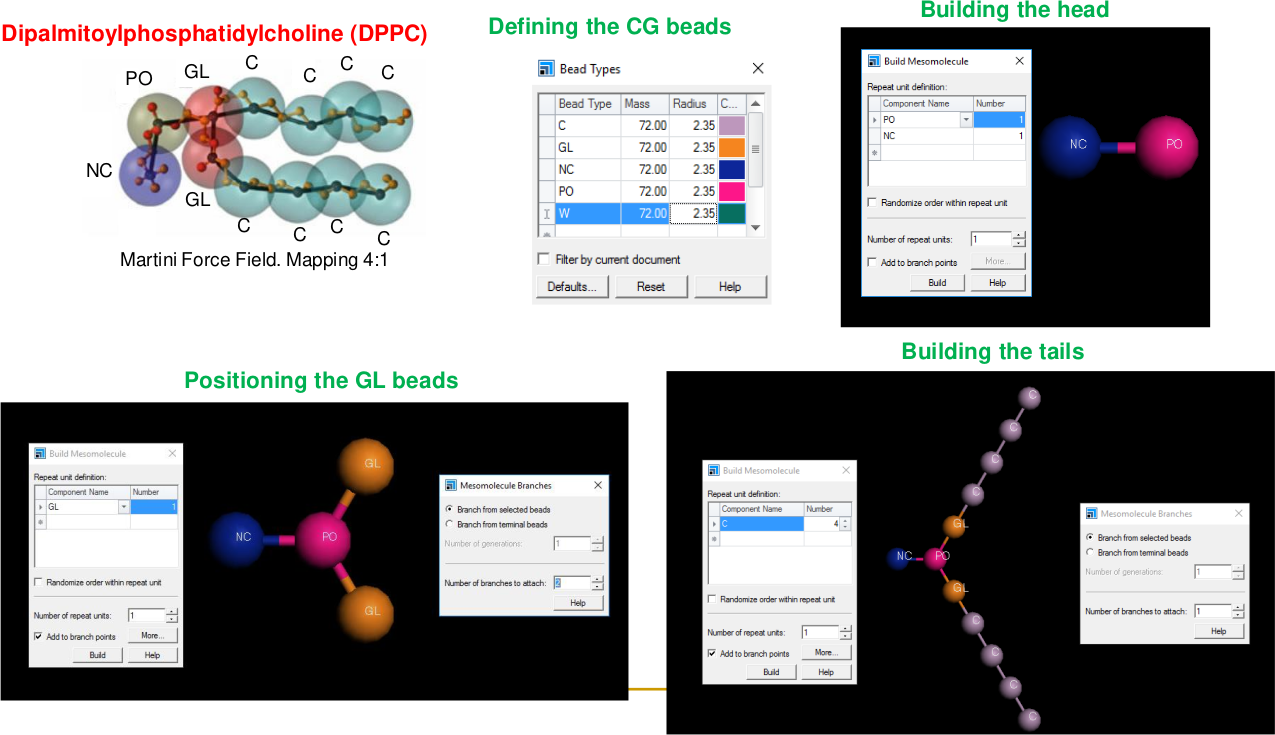
\includegraphics[height=2.31in,width=4.00in,viewport=0 0 1275 735,clip]{Figures/MS-Building_Mesomolecule.png}
\caption{\tiny \textrm{Building Meso-molecule structure for Materials studio.}}%(与文献\cite{EPJB33-47_2003}图1对比)
\label{MS-Building_Meso-molecules}
\end{figure}
}

\frame
{
	\frametitle{\textrm{MS~Modelling:~Meso-molecules by template}}
\begin{figure}[h!]
\centering
\vspace*{-0.12in}
\includegraphics[height=2.36in,width=4.00in,viewport=0 0 1224 720,clip]{Figures/MS-Building_Mesomolecule-template.png}
\caption{\tiny \textrm{Building Meso-molecule by temlapte for Materials studio.}}%(与文献\cite{EPJB33-47_2003}图1对比)
\label{MS-Building_Meso-molecules-template}
\end{figure}
}

\frame
{
	\frametitle{\textrm{MS~Modelling:~Meso-molecules by template}}
\begin{figure}[h!]
\centering
\vspace*{-0.18in}
\includegraphics[height=2.70in,width=3.72in,viewport=0 0 1133 822,clip]{Figures/MS-Building_Mesomolecule-example.png}
\caption{\tiny \textrm{Building Meso-molecule by temlapte for Materials studio.}}%(与文献\cite{EPJB33-47_2003}图1对比)
\label{MS-Building_Meso-molecules-template-example}
\end{figure}
}

\frame
{
	\frametitle{\textrm{MS~Modelling:~MOF Crystals}}
\begin{figure}[h!]
\centering
\vspace*{-0.18in}
\includegraphics[height=2.60in,width=4.00in,viewport=0 0 1148 740,clip]{Figures/MS-Building_MOF.png}
\caption{\tiny \textrm{Building Metal Framework Orgainc (MOF) for Materials studio.}}%(与文献\cite{EPJB33-47_2003}图1对比)
\label{MS-Building_MOF}
\end{figure}
}

\frame
{
	\frametitle{\textrm{MS~Modelling:~Miller Planes in Crystals}}
\begin{figure}[h!]
\centering
\vspace*{-0.18in}
\includegraphics[height=2.60in,width=4.00in,viewport=0 0 880 569,clip]{Figures/MS-Building_Miller_Plane.png}
\caption{\tiny \textrm{Building Miller Planes in crystals for Materials studio.}}%(与文献\cite{EPJB33-47_2003}图1对比)
\label{MS-Building_Miller-Plane}
\end{figure}
}

\frame
{
	\frametitle{\textrm{MS~Modelling:~surface from Crystals}}
\begin{figure}[h!]
\centering
\vspace*{-0.10in}
\includegraphics[height=2.20in,width=4.00in,viewport=0 0 1349 724,clip]{Figures/MS-Building_Cleave_Surface.png}
\caption{\tiny \textrm{Building surfaces from crystals for Materials studio.}}%(与文献\cite{EPJB33-47_2003}图1对比)
\label{MS-Building_Cleave_Surface}
\end{figure}
}

\frame
{
	\frametitle{\textrm{MS~Modelling:~surface in Crystals}}
\begin{figure}[h!]
\centering
\vspace*{-0.18in}
\includegraphics[height=2.70in,width=3.90in,viewport=0 0 1064 737,clip]{Figures/MS-Building_Surface.png}
\caption{\tiny \textrm{Building surfaces in crystals for Materials studio.}}%(与文献\cite{EPJB33-47_2003}图1对比)
\label{MS-Building_Surface}
\end{figure}
}

\frame
{
	\frametitle{\textrm{MS~Modelling:~layers and vacuum}}
\begin{figure}[h!]
\centering
\vspace*{-0.18in}
\includegraphics[height=2.70in,width=3.60in,viewport=0 0 1006 763,clip]{Figures/MS-Building_layer.png}
\caption{\tiny \textrm{Building metal-polymer-metal by multi-layers and vacuum for Materials studio.}}%(与文献\cite{EPJB33-47_2003}图1对比)
\label{MS-Building_layer}
\end{figure}
}

\section{\rm{Materials~Studio}:~计算}
\frame
{
	\frametitle{\textrm{Quantum simulation:~Tools}}
\begin{figure}[h!]
\centering
\vspace*{-0.10in}
\includegraphics[height=2.10in,width=4.00in,viewport=0 0 1459 763,clip]{Figures/MS-Quantum_simulation-tools.png}
\caption{\tiny \textrm{Calculation modules for quantum simulation in Materials studio.}}%(与文献\cite{EPJB33-47_2003}图1对比)
\label{MS-Quantum_simulation}
\end{figure}
}

\frame
{
	\frametitle{\textrm{MS~Calculation modules comparison}}
\begin{figure}[h!]
\centering
\vspace*{-0.10in}
\includegraphics[height=1.60in,width=4.00in,viewport=0 0 1517 602,clip]{Figures/MS-Caluculator-compare-1.png}
\caption{\tiny \textrm{Calculation parameters comparison in Materials studio.}}%(与文献\cite{EPJB33-47_2003}图1对比)
\label{MS-Module_parameters}
\end{figure}
}

\frame
{
	\frametitle{\textrm{MS~xc functional  comparison}}
\begin{figure}[h!]
\centering
\vspace*{-0.15in}
\includegraphics[height=2.40in,width=4.00in,viewport=0 0 1261 751,clip]{Figures/MS-xc_functional-compare.png}
\caption{\tiny \textrm{XC functional comparison in Materials studio.}}%(与文献\cite{EPJB33-47_2003}图1对比)
\label{MS-Module_xc-functional}
\end{figure}
}

\frame
{
	\frametitle{\textrm{MS~Calculation modules comparison}}
\begin{figure}[h!]
\centering
\vspace*{-0.18in}
\includegraphics[height=2.70in,width=3.60in,viewport=0 0 969 728,clip]{Figures/MS-Caluculator-compare-2.png}
\caption{\tiny \textrm{Calculation modules comparison in Materials studio.}}%(与文献\cite{EPJB33-47_2003}图1对比)
\label{MS-Module_xc-functional}
\end{figure}
}

\frame
{
	\frametitle{\textrm{MS~Calculation:~ONETEP}}
\begin{figure}[h!]
\centering
\vspace*{-0.12in}
\includegraphics[height=2.15in,width=2.14in,viewport=0 0 646 650,clip]{Figures/MS-Caluculator_ONETEP-parameter.png}
\includegraphics[height=2.15in,width=1.68in,viewport=0 0 605 776,clip]{Figures/MS-Caluculator_ONETEP-analysis.png}
\caption{\tiny \textrm{Calculation module ONETEP in Materials studio.}}%(与文献\cite{EPJB33-47_2003}图1对比)
\label{MS-Calculation_ONETEP}
\end{figure}
}

\frame
{
	\frametitle{\textrm{MS~Calculation:~DFTB+ \& VAMP}}
\begin{figure}[h!]
\centering
\vspace*{-0.15in}
\includegraphics[height=2.00in,width=1.90in,viewport=0 0 635 671,clip]{Figures/MS-Caluculator_DFTB-parameter.png}
\includegraphics[height=2.00in,width=1.96in,viewport=0 0 723 739,clip]{Figures/MS-Caluculator_VAMP-parameter.png}
\caption{\tiny \textrm{Calculation parameters for module DFTB+ and VAMP in Materials studio.}}%(与文献\cite{EPJB33-47_2003}图1对比)
\label{MS-Calculation_DFTB-VAMP}
\end{figure}
}

\frame
{
	\frametitle{\textrm{MS~Calculation:~QMERA}}
\begin{figure}[h!]
\centering
\vspace*{-0.18in}
\includegraphics[height=2.58in,width=4.00in,viewport=0 0 1161 746,clip]{Figures/MS-Caluculator_QMERA-parameter.png}
\caption{\tiny \textrm{Calculation parameters for module QMERA in Materials studio.}}%(与文献\cite{EPJB33-47_2003}图1对比)
\label{MS-QMERA}
\end{figure}
}

\frame
{
	\frametitle{\textrm{Classical simulation:~Tools}}
\begin{figure}[h!]
\centering
\vspace*{-0.10in}
\includegraphics[height=1.91in,width=4.00in,viewport=0 0 1494 711,clip]{Figures/MS-Classical_simulation-tools.png}
\caption{\tiny \textrm{Calculation modules for classical simulation in Materials studio.}}%(与文献\cite{EPJB33-47_2003}图1对比)
\label{MS-Classical_simulation-}
\end{figure}
}

\frame
{
	\frametitle{\textrm{MS~Calculation:~Forcite}}
\begin{figure}[h!]
\centering
\vspace*{-0.18in}
\includegraphics[height=2.70in,width=3.08in,viewport=0 0 845 741,clip]{Figures/MS-Caluculator_Forcite-parameter.png}
\caption{\tiny \textrm{Calculation modules Forcite in Materials studio.}}%(与文献\cite{EPJB33-47_2003}图1对比)
\label{MS-Forcite_Plus}
\end{figure}
}

\frame
{
	\frametitle{\textrm{MS~Calculation:~Adsorption Lactor}}
\begin{figure}[h!]
\centering
\vspace*{-0.18in}
\includegraphics[height=2.67in,width=4.00in,viewport=0 0 1093 728,clip]{Figures/MS-Caluculator_Adsorption-Lactor-example.png}
\caption{\tiny \textrm{Calculation modules Adsorption Lactor in Materials studio.}}%(与文献\cite{EPJB33-47_2003}图1对比)
\label{MS-Adsorption_Lactor}
\end{figure}
}

\frame
{
	\frametitle{\textrm{MS~Calculation:~Amorphous Cell}}
\begin{figure}[h!]
\centering
\vspace*{-0.18in}
\includegraphics[height=2.67in,width=2.53in,viewport=0 0 702 750,clip]{Figures/MS-Caluculator_Amorphous-Cell-parameter.png}
\caption{\tiny \textrm{Calculation modules Amorphous cell in Materials studio.}}%(与文献\cite{EPJB33-47_2003}图1对比)
\label{MS-Amorphous_cell}
\end{figure}
}

\frame
{
	\frametitle{\textrm{MS~Calculation:~Blends}}
\begin{figure}[h!]
\centering
\vspace*{-0.14in}
\includegraphics[height=2.43in,width=4.00in,viewport=0 0 1358 822,clip]{Figures/MS-Caluculator_Blends-example.png}
\caption{\tiny \textrm{Calculation modules Blends in Materials studio.}}%(与文献\cite{EPJB33-47_2003}图1对比)
\label{MS-Blends}
\end{figure}
}

\frame
{
	\frametitle{\textrm{MS~Calculation:~Conformers}}
\begin{figure}[h!]
\centering
\vspace*{-0.14in}
\includegraphics[height=2.33in,width=4.00in,viewport=0 0 1278 743,clip]{Figures/MS-Caluculator_Conformers-parameter.png}
\caption{\tiny \textrm{Calculation modules Conformers in Materials studio.}}%(与文献\cite{EPJB33-47_2003}图1对比)
\label{MS-Conformer}
\end{figure}
}

\frame
{
	\frametitle{\textrm{Mesoescale simulation:~Tools}}
\begin{figure}[h!]
\centering
%\vspace*{-0.10in}
\includegraphics[height=1.40in,width=4.00in,viewport=0 0 1391 482,clip]{Figures/MS-Mesoescale_simulation-tools.png}
\caption{\tiny \textrm{Calculation modules for mesoescale simulation in Materials studio.}}%(与文献\cite{EPJB33-47_2003}图1对比)
\label{MS-Mesoescale_simulation-}
\end{figure}
}

\frame
{
	\frametitle{\textrm{MS~Calculation:~Mesocite}}
\begin{figure}[h!]
\centering
%\vspace*{-0.14in}
\includegraphics[height=1.65in,width=4.00in,viewport=0 0 1188 488,clip]{Figures/MS-Caluculator_Mesocite-parameter.png}
\caption{\tiny \textrm{Calculation modules Mesocite in Materials studio.}}%(与文献\cite{EPJB33-47_2003}图1对比)
\label{MS-Mesocite}
\end{figure}
}

\section{\rm{Materials~Studio}:~分析}
\frame
{
	\frametitle{\textrm{MS~Analytical and crystallization tools}}
\begin{figure}[h!]
\centering
\vspace*{-0.18in}
\includegraphics[height=2.70in,width=2.61in,viewport=0 0 850 821,clip]{Figures/MS-Analysis-cry_tools.png}
\caption{\tiny \textrm{Analytical and crystallization tools in Materials studio.}}%(与文献\cite{EPJB33-47_2003}图1对比)
\label{MS-Analysis-cry}
\end{figure}
}

\frame
{
	\frametitle{\textrm{MS~Analysis:~Reflex}}
\begin{figure}[h!]
\centering
%\vspace*{-0.14in}
\includegraphics[height=1.36in,width=4.00in,viewport=0 0 1374 467,clip]{Figures/MS-Analysis_Reflex.png}
\caption{\tiny \textrm{Analysis module Reflex overview in Materials studio.}}%(与文献\cite{EPJB33-47_2003}图1对比)
\label{MS-Analysis-Reflex-overview}
\end{figure}
}

\frame
{
	\frametitle{\textrm{MS~Analysis:~Reflex}}
\begin{figure}[h!]
\centering
\vspace*{-0.14in}
\includegraphics[height=2.47in,width=4.00in,viewport=0 0 1256 775,clip]{Figures/MS-Analysis_Reflex-example.png}
\caption{\tiny \textrm{Reflex pattern processing in Materials studio.}}%(与文献\cite{EPJB33-47_2003}图1对比)
\label{MS-Analysis-Reflex-example-1}
\end{figure}
}

\frame
{
	\frametitle{\textrm{Reflex:~Pattern Processing}}
\begin{figure}[h!]
\centering
\vspace*{-0.10in}
\includegraphics[height=1.63in,width=4.00in,viewport=0 0 1349 548,clip]{Figures/MS-Analysis_Reflex_Pattern-Processing.png}
\caption{\tiny \textrm{Pattern Processing parameters in Materials studio.}}%(与文献\cite{EPJB33-47_2003}图1对比)
\label{Reflex-Pattern-Processing}
\end{figure}
}

\frame
{
	\frametitle{\textrm{MS~Analysis:~Reflex}}
\begin{figure}[h!]
\centering
\vspace*{-0.14in}
\includegraphics[height=2.41in,width=4.00in,viewport=0 0 1270 764,clip]{Figures/MS-Analysis_Reflex_Powder-Diffraction-example.png}
\caption{\tiny \textrm{Reflex powder diffraction in Materials studio.}}%(与文献\cite{EPJB33-47_2003}图1对比)
\label{MS-Analysis-Reflex-example-2}
\end{figure}
}

\frame
{
	\frametitle{\textrm{Reflex:~Powder Diffraction}}
\begin{figure}[h!]
\centering
\vspace*{-0.10in}
\includegraphics[height=1.92in,width=4.00in,viewport=0 0 1343 644,clip]{Figures/MS-Analysis_Reflex_Powder-Diffraction-1.png}
\caption{\tiny \textrm{Powder Diffraction parameters in Materials studio.}}%(与文献\cite{EPJB33-47_2003}图1对比)
\label{Reflex-Powder_Diffraction-1}
\end{figure}
}

\frame
{
	\frametitle{\textrm{Reflex:~Powder Diffraction}}
\begin{figure}[h!]
\centering
\vspace*{-0.10in}
\includegraphics[height=1.70in,width=4.00in,viewport=0 0 1342 569,clip]{Figures/MS-Analysis_Reflex_Powder-Diffraction-2.png}
\caption{\tiny \textrm{Powder Diffraction parameters in Materials studio.}}%(与文献\cite{EPJB33-47_2003}图1对比)
\label{Reflex-Powder_Diffraction-2}
\end{figure}
}

\frame
{
	\frametitle{\textrm{Reflex:~Powder Indexing}}
\begin{figure}[h!]
\centering
\vspace*{-0.10in}
\includegraphics[height=1.63in,width=4.00in,viewport=0 0 1349 548,clip]{Figures/MS-Analysis_Reflex_Powder-Indexing.png}
\caption{\tiny \textrm{Powder Indexing parameters in Materials studio.}}%(与文献\cite{EPJB33-47_2003}图1对比)
\label{Reflex-Powder-Indexing}
\end{figure}
}

\frame
{
	\frametitle{\textrm{Reflex:~Powder Refinement}}
\begin{figure}[h!]
\centering
\vspace*{-0.18in}
\includegraphics[height=2.70in,width=2.30in,viewport=0 0 620 732,clip]{Figures/MS-Analysis_Reflex_Powder-Refinement.png}
\caption{\tiny \textrm{Powder Refinement parameters in Materials studio.}}%(与文献\cite{EPJB33-47_2003}图1对比)
\label{Reflex-Powder-Refinement}
\end{figure}
}

\frame
{
	\frametitle{\textrm{Reflex:~Powder QPA}}
\begin{figure}[h!]
\centering
%\vspace*{-0.18in}
\includegraphics[height=1.92in,width=4.00in,viewport=0 0 1296 621,clip]{Figures/MS-Analysis_Reflex_Powder-QPA.png}
\caption{\tiny \textrm{Powder QPA parameters in Materials studio.}}%(与文献\cite{EPJB33-47_2003}图1对比)
\label{Reflex-Powder-QPA}
\end{figure}
}

\frame
{
	\frametitle{\textrm{MS~Analysis:~Morphology}}
\begin{figure}[h!]
\centering
\vspace*{-0.18in}
\includegraphics[height=2.70in,width=3.06in,viewport=0 0 817 722,clip]{Figures/MS-Crystallization-example.png}
\caption{\tiny \textrm{Example:~Morphology calculation in Materials studio.}}%(与文献\cite{EPJB33-47_2003}图1对比)
\label{MS-Morphology}
\end{figure}
}


